\documentclass[a4j,12pt]{jarticle}
\usepackage[dvipdfmx]{graphicx,color}
\usepackage{epsfig,here}
\usepackage{caption}
\usepackage{url}
\usepackage{bm}
\usepackage{tikz}
\usepackage{scalefnt}
\usepackage{amsmath,amssymb}
\usepackage{amsthm}
\usepackage{ascmac}
\usepackage{latexsym}
\newtheorem{dfn}{定義}[section]
\newtheorem{thm}{定理}[section]
\newtheorem{lem}{補題}[section]
\renewcommand{\proofname}{\bfseries 証明}
\usetikzlibrary{decorations.pathreplacing}
\usetikzlibrary{shadows}
\begin{document}
\begin{center}
	{\LARGE アローの不可能性定理}\\
	\vspace{.5em}
    〜架空世界の社会的決定について考える〜\\
	{\large \lineskip .8em
		\begin{tabular}[t]{c}
		    @nymwa
        \end{tabular}
		\par}
		\vskip .5em
	{\large 平成30年3月8日}
\end{center}

\section{民主的な決定は難しい}
我々はしばしば,「みんなで何かを決める」という状況に直面することがあります.例えば,友人と一緒にいて「今日の昼ご飯,何を食べようか?」などとなることがあるかもしれません.今仮に,Lupaくん,Maxeくん,Nymwaくんの3人が昼ご飯に何を食べに行くか相談しているとしましょう.それぞれの人は以下のように主張しました.
\begin{align*}
    Lupa &「私は牛丼が食べたい.その次にカレー.ラーメンは別にいいや.」\\
    Maxe &「僕はカレーが食べたい.別にラーメンでもいいけど.牛丼はいいや.」\\
    Nymwa &「ラーメン自明.牛丼は許す.カレー?アリエナイ…」
\end{align*}
みんなバラバラの意見になってしまいました.このままでは昼ご飯が食べられないので,Nymwaくんが残りの2人にこう聞きました.
\begin{align*}
    Nymwa &「みんな,牛丼とカレーならどっちがいい?」
\end{align*}
LupaくんとNymwaくんは,カレーより牛丼を食べたがっています.一方Maxeくんはカレーが食べたい.多数決を取ったところ,2対1でカレーよりは牛丼ということになりました.Nymwaくんはさらに聞きます.
\begin{align*}
    Nymwa &「じゃあ,牛丼とラーメンならどっちがいい?」
\end{align*}
MaxeくんとNymwaくんは,牛丼よりラーメンが食べたいです.Lupaくんは逆なので,これもまた2対1で牛丼よりラーメンということになります.
\begin{align*}
    Nymwa &「1位ラーメン,2位牛丼,3位カレー,ラーメン食べよう.」
\end{align*}
Nymwaくんはラーメンが食べられると思って非常に喜びました.しかし,ここでLupaくんが言いました.
\begin{align*}
    Lupa &「ラーメンとカレーならどっちがいい?」
\end{align*}
すると,2対1で「カレーはラーメンよりも良い」ということになってしまいます.3位のカレーは1位のラーメンより良い.あれ?

このように選択肢の取りうるペアすべてに対して多数決を取った場合,選択肢の間で「ラーメン > 牛丼 > カレー > ラーメン$\dots\dots$」と堂々巡りが起こることがあります.これを「投票のパラドックス」とか「コンドルセのパラドックス」と言います.

Lupaくんの提案によって,このようなパラドックスが生じてしまったわけなのですが,もしLupaくんがNymwaくんのラーメン推しに何も文句を付けなかった場合,実際に3人はラーメンを食べに行っていたかもしれません.しかし,その場合3人中2人は「ラーメンよりはカレーの方が良い」のであって,「カレーではなくラーメンを選ぶ」というこの3人の集団的な決定に対しては,意思を同じくする個人がNymwaくんただ一人になってしまいます.つまり,Nymwaくんはこの集団の意思決定において,「他の誰がなんと言おうがラーメンは他の選択肢よりも良い」と決めさせる「独裁者」となっているとも言えます.果たしてこれは「民主的な決定」と言えるのでしょうか.

このような決め方の手法には,どうも多数のパラドックスが見つかっているそうです.では,民主的と言えて,かつ堂々巡りの起きないような決め方の方式というのは存在するのでしょうか.


\section{準備}
集団がいくつかの選択肢に順位付け・ランク付け(同率を許す)をするという状況を考えてみましょう.今仮に,ある国で今年の人気歌手ランキングを作ることになったとします.さて,どのように作成すればいいでしょうか.

もしもその国のすべての人の各歌手への好感度を測定することができるとしたら,好感度の和が高い順に順位を付けていけば良いのかもしれません.しかし,「○○さんは10好きだけど,××さんは3好きだなぁー.」などと,個人の好き嫌いの度合いを量的な尺度で扱うのは無理がありそうです.

そこで,一人ひとりに「あなたの好きな歌手ランキング」を書いてもらって,集計して最終的な国全体のランキングを作成することにしました.しかし,そのようにして集められた結果から一体どのようにして,それぞれの歌手の間に順位付けをすればいいのでしょうか.というか,そもそも順位ってなんなんでしょうか.

まずは,議論に必要な言葉や記号を定義していきましょう\footnote{これ以降で出てくる用語には私がかってに命名したものもあるので,広く使われているものとは限らないことに注意してください.}.

\subsection{選択肢と選好}
\begin{dfn}
    選択肢とは,個人や社会がその価値判断に基づいて評価し,選択したり順序付けたりする対象のことです.
\end{dfn}
\begin{dfn}
    選好とは,ある選択肢が他の選択肢よりも「良い」という判断のことです.個人の選好を個人的選好,その人たちが属する社会の選好を社会的選好と言います.
\end{dfn}

どのような決定方法でも選択肢と,それを選ぶ人は存在します.選択肢は人かもしれませんし,社会の状態かもしれませんし,いろいろです.選ぶ人は自分の判断,すなわち選好に基づいて選択肢を選んだり拒んだりします.

以降,選択肢(Alternatives)全体の集合を$A$,個人をラテン文字の小文字$i,j,k,\dots$で表し,社会に属する全個人の集合を$M$,その部分集合を$V,W,\dots$と表します.$M$はmembersのつもりです.また,選択肢,個人の数は有限とします.

\subsection{記号の定義}
この文書全体で用いられる集合や論理の記号の意味を説明します.なお,命題とは真か偽か判断できる文のことです.
\begin{itemize}
    \item[$\sim$]
        否定.「$\sim P$」は,「Pではない」という命題です.
    \item[$\land$]
        論理積.「$P \land Q$」は,「PとQがともに真である」という命題です.
    \item[$\lor$]
        論理和.「$P \lor Q$」は,「PとQの少なくとも片方は真である」という命題です.
    \item[$\to$]
        含意.「$P \to Q$」は,「PとQはともに真,あるいはPは偽である」,すなわち「PならばQ」という命題です.
    \item[$\leftrightarrow$]
        同値.「$P \leftrightarrow Q$」は,「PとQはともに真,あるいはともに偽」という命題です.
    \item[$\in$]
        属する.「$x \in X$」は,「要素$x$は集合$X$に属する」という意味です.
    \item[$\subset$]
        部分集合,含まれる.「$A \subset B$」は,「集合Aは集合Bに含まれる」という意味です.「$B \supset A$」はこれと同じです.
    \item[$-$]
        差集合.$A-B$で集合AからBの要素を取り除いた集合を意味します.
    \item[$|A|$]
        要素数.$|A|$で集合Aに属する要素数を意味します.
    \item[$A^n$]
        $A$の直積.$A$の要素のnつ組の集合です.$R^2$は平面になります.
    \item[$2^A$]
        べき集合.$2^A$で集合Aのすべての部分集合からなる集合を意味します.
    \item[$\exists$]
        存在量化子.「$\exists x \in X \: P(x)$」は,「集合Xの中にはある要素xが存在して命題P(x)が満たされる」という命題です.    
    \item[$\forall$]
        全称量化子.「$\forall x \in X \: P(x)$」は,「集合Xの中のすべての要素xに対して命題P(x)が成立する」という命題です.
\end{itemize}

論理記号の結合の優先度は$\sim,\exists,\forall$が最も高く,次に$\land,\lor$で,$\to,\leftrightarrow$が最も低いです.$P \to Q \to R$や$P \leftrightarrow Q \leftrightarrow R$は,それぞれ$(P \to Q) \land (Q \to R)$,$(P \leftrightarrow Q) \land (Q \leftrightarrow R)$を意味します.左寄せ・右寄せの規則等は設けません.

\subsection{二項関係}
\begin{dfn}
    集合$X$上の二項関係$R$とは,集合$X^2$上で定義され,任意の$x,y \in X$に対して命題$xRy$が真か偽かを定める関数です.$xRy$が真であることを$xRy$,偽であることを$\sim xRy$または$x\not \! \! R y$と表します.
\end{dfn}

$X = \{グー,チョキ,パー\}$.$X$上の二項関係$xRy$を「xがyに勝つ」とします.このとき,「グー$R$チョキ」,「チョキ$R$パー」,「パー$R$グー」ですが,その他の組み合わせ(負けorあいこ)では例えば「グー$\not \! \! R$パー」です.

選択肢間の選好は,選択肢の集合$A$上の二項関係として表現できます.
\begin{dfn}
    選択肢$x$と$y$に対して,$x \ge y$は,「xはyと少なくとも同じぐらいよい」とする二項関係です.
\end{dfn}
「xはyと少なくとも同じぐらいよい」というのは「xとyが同じぐらい良いか,または明確にxはyよりも良い」という意味であることに気をつけてください.また,$\ge$が意味的に対応していることを確認してください.

\begin{dfn}
    $\ge$の右下に個人または個人の集合を$x \ge_i y$,$x \ge_V y$とつけた場合,それぞれ,「個人$i$は,xはyと少なくとも同じぐらいよいと選好する」,「集合$V$に含まれるすべての個人$j$が,xはyと少なくとも同じぐらいよいと選好する」という二項関係です.
\end{dfn}

\begin{dfn}
    $x \succeq y$は,「社会的にxはyと少なくとも同じぐらいよい」と選好するという二項関係です.
\end{dfn}

「$\succeq$なんて見たことないしぐにゃってしてて怖いよぅ」などとして読むのを止めないでほしいです\footnote{昔の自分はそうでした.}.

$x \ge_M y$と$x \succeq y$が全く異なるものを意味していることに注意してください.$x \ge_M y$は「社会に属するすべての個人が"$x \ge y$"と思っている」ですが,$x \succeq y$は「社会全体では"$x \ge y$"というように決まった」という意味です.これは,例えばある事案で賛否を取ったとき,全ての個人が賛成したのなら社会的にも賛成となるのでしょうが,社会的に賛成だとしても社会の中には反対とした個人がいるかもしれないという違いです.

二項関係$>,<,\doteq,\succ,\prec,\simeq$を以下のように定義します.
\begin{dfn}
    $x>y \leftrightarrow (x \geq y かつ y \not \geq x) \leftrightarrow y<x$
\end{dfn}
\begin{dfn}
    $x \doteq y \leftrightarrow (x \geq y かつ y \geq x)$
\end{dfn}
\begin{dfn}
    $x \succ y \leftrightarrow (x \succeq y かつ y \not \succeq x) \leftrightarrow y \prec x$
\end{dfn}
\begin{dfn}
    $x \simeq y \leftrightarrow (x \succeq y かつ y \succeq x)$
\end{dfn}

$x>y$は「xはyよりも明確に良い」,すなわち,「xをyよりも選好する」という意味になります.

$x\doteq y$は,「xとyは同程度によい」という意味ですが,「xとyはどちらのほうが良いとも言えない」という意味ではないことに注意してください.$x$と$y$が取れる選好は以下の4つにいずれかになり,
\begin{align*}
    1 :& x \geq y かつ y \geq x \hspace{1em} (x \doteq y) \\
    2 :& x \geq y かつ y \not \geq x \hspace{1em} (x > y) \\
    3 :& x \not \geq y かつ y \geq x \hspace{1em} (x < y) \\
    4 :& x \not \geq y かつ y \not \geq x \hspace{1em} 
\end{align*}
「xとyはどちらのほうが良いとも言えない」はこのうち4番目です.ただ,後で出てくる「完全性」の制約のために4番目の場合に注意する必要はあまりないので安心してください.

また,$x\doteq y$は,「$x$と$y$が同一の選択肢である」という意味ではないことにも注意してください.この場合,$x$と$y$は,同じ選択肢かもしれませんし,異なる選択肢かもしれません.$\doteq$が等しいとしているのはその個人が評価する選択肢の価値です.また,$\doteq$の上の点を付けた理由は$=$との混同を防ぐためです.

\subsection{二項関係$\geq$や$\succeq$が満たす性質}
先程定義した$\geq$では,例えば$x \not \geq x$としたとき,「xはxより良いとは言えない」という意味になってしまい,不思議な選好になってしまいます.これから議論する選好がこのようにならないために,満たしてほしい性質をいくつか決める必要があります.
\begin{dfn}[反射性]
    任意の二項関係$R$は,すべての選択肢$x$に対し,$x R x$を満たすとき反射性を持つと言います.
\end{dfn}
\begin{dfn}[完全性]
    任意の二項関係$R$は,任意の{\bf 異なる\footnote{この「異なる」がないと,$xRx$のような場合も含むため反射性の条件を包含してしまいます.}}2つの選択肢のペアx,yに対し,$x R y \lor y R x$を満たすとき完全性を持つと言います.完全性は比較可能性とも言います.
\end{dfn}
\begin{dfn}[推移性]
    任意の二項関係$R$は,任意の3つの選択肢の組x,y,zに対して,$x R y \land y R z \to x R z$を満たすとき推移性を持つと言います.
\end{dfn}
\begin{dfn}
    弱順序とは,反射性,完全性,推移性をすべて満たす二項関係のことです.
\end{dfn}

反射性によって$x \not \geq x$のような事態は回避されます.

完全性が満たされているというのは,さきほどの4パターンのうち4番目の「どちらが良いとも言えない」というパターンはないということです.人気歌手アンケートの回答で言えば,「この人とこの人は毛色が違いすぎて優劣もなにもそもそも比較できないし,順位なんて付けられない」という回答は考えないということになります.

推移性は,「xがyより好きで,yがzより好きなら,当然xがzより好き」という自然そうな性質です.また,推移性のおかげで「コンドルセのパラドックス」の$x > y$かつ$y > z$かつ$z > x$のような選択肢間で循環が起こるおかしな選好が許されなくなります.理由は図2の例に推移性を適用ができるかを調べて確認してください.

以下に弱順序とそうでないものの例をそれぞれ図1,図2に挙げておきます.矢印「$x \leftarrow y$」は$x\geq y$の関係があることを表しています.両矢印は$\doteq$です.また,反射性は当然成り立つものとし,自分自身との関係については省略しました.
\begin{figure}[!h]
    \centering
    \begin{minipage}{0.55\hsize}
    {\scalefont{0.9}
        \begin{tikzpicture}
            \node (1) at (1,2) {桃};
            \node (2) at (0,0) {栗};
            \node (3) at (2,0) {柿};
            \draw [thick, <-] (1) -> (2);
            \draw [thick, <-] (1) -> (3);
            \draw [thick, <-] (2) -> (3);
        \end{tikzpicture}
        \begin{tikzpicture}
            \node (1) at (1,2) {桃};
            \node (2) at (0,0) {栗};
            \node (3) at (2,0) {柿};
            \draw [thick, <->] (1) -> (2);
            \draw [thick, <->] (1) -> (3);
            \draw [thick, <->] (2) -> (3);
        \end{tikzpicture}
        \begin{tikzpicture}
            \node (1) at (0,2) {犬};
            \node (2) at (2,2) {猫};
            \node (3) at (0,0) {鳥};
            \node (4) at (2,0) {魚};
            \draw [thick, ->] (1) -> (2);
            \draw [thick, <-] (1) -> (3);
            \draw [thick, <->](1) -> (4);
            \draw [thick, <-] (2) -> (3);
            \draw [thick, <-] (2) -> (4);
            \draw [thick, ->] (3) -> (4);
        \end{tikzpicture}}
        \caption{弱順序}
    \end{minipage}
    \begin{minipage}{0.4\hsize}
    {\scalefont{0.9}
        \begin{tikzpicture}
            \node (1) at (1,2) {桃};
            \node (2) at (0,0) {栗};
            \node (3) at (2,0) {柿};
            \draw [thick, <-] (1) -> (2);
            \draw [thick, ->] (1) -> (3);
            \draw [thick, <-] (2) -> (3);
        \end{tikzpicture}
        \begin{tikzpicture}
            \node (1) at (0,2) {犬};
            \node (2) at (2,2) {猫};
            \node (3) at (0,0) {鳥};
            \node (4) at (2,0) {魚};
            \draw [thick, ->] (1) -> (2);
            \draw [thick, <-] (1) -> (3);
            \draw [thick, <-] (2) -> (3);
            \draw [thick, <-] (2) -> (4);
            \draw [thick, ->] (3) -> (4);
        \end{tikzpicture}}
        \caption{弱順序でない}    
    \end{minipage}
\end{figure}

図1の一番左の三角形を見てください.この例では「$桃 > 栗 > 柿$」と選好しています.真ん中の例では「$桃\doteq 栗\doteq 柿$」と全て同率1位,右の例では「$猫>犬\doteq 魚>鳥$」で猫1位,犬・魚同率2位,鳥3位と順位がつけられます.

しかし,図2の左の例では循環してしまっています.「桃より柿,柿より栗,栗より桃が好き」などと言うものを個人的選好として扱うのは少し厳しいような気がします.また,右の例では犬と魚の順位が比較できません.このように選択肢間で比較できないとするようなものも個人的選好として許してしまうと色々と大変です.この例では実感がわきませんが,選択肢「平家物語」と「有楽町駅」で比較しろと言われても困るように,選択肢間で比較できるものだけに限るという条件は大切です.

以上の理由から,以降個人的選好・社会的選好が当然満たしている性質として弱順序を仮定することにします.特に断りがなければ$\ge,\succeq$は弱順序ですし,選好と言ったら弱順序です\footnote{と,ここでは言ってますが,5章で推移性を満たさない選好についても考えます.}.

選好を弱順序に制限することが不自然に思えるかもしれませんが,それについては第5章で少し触れることにします.

\subsection{厚生関数}
今まで選好の二項関係を用いた表し方について見てきました.次に,個人的選好から社会的選好を決めることについて考えます.個人的選好にも様々なものが考えられます.例えば,個人$i$の3選択肢$x,y,z$に対する個人的選好は,以下に示す13通りのうちのどれかになります.各自選好がこれのみに限られることを確認してください\footnote{ちなみに,n選択肢に対する個人的選好の数は$n=1$から,$1,3,13,75,541,\dots$と増えていきます.この数列を順序付きベル数,フビニ数と言います.}.
\begin{equation*}
\begin{array}[h]{cccccc}
    1 : & x > y > z &
    2 : & y > z > x &
    3 : & z > x > y \\
    4 : & x > z > y &
    5 : & y > x > z &
    6 : & z > y > x \\
    7 : & x > y \doteq z &
    8 : & y > z \doteq x &
    9 : & z > x \doteq y \\
    10: & x \doteq y > z &
    11: & y \doteq z > x &
    12: & z \doteq x > y \\
    13: & x \doteq y \doteq z & & & &
\end{array}
\end{equation*}

さて,個人$i$の個人的選好を代入できる変数を$P_i$と書くことにし,個人的選好と社会的選好を対応させる関数について考えます.

\begin{dfn}[厚生関数]
    n人の個人的選好$P_i$の組$(P_1,P_2,P_3,\dots,P_n)$に対して,社会的選好$P$を1通りに定める関数を厚生関数と言います.
\end{dfn}
例えば,最初に出てきた昼ご飯の例で,Nymwaくんの意見が採用された場合を考えると,各個人と社会の選好は,
\begin{eqnarray*}
    \begin{array}[h]{ccl}
        P_{Lupa}  &=& 牛丼 > カレー > ラーメン \\
        P_{Maxe}  &=& カレー > ラーメン > 牛丼 \\
        P_{Nymwa} &=& ラーメン > 牛丼 > カレー \\
        P &=& ラーメン \succ 牛丼 \succ カレー \\
    \end{array}\\
\end{eqnarray*}
となり,"牛丼vs.カレー"の後,"勝者vs.ラーメン"と多数決を取っていく厚生関数をfとすると,$P = f(P_{Lupa},P_{Maxe},P_{Nymwa})$と書けます.

厚生関数に代入したり出力される選好は弱順序なので,例えば$P_i$や$P$に"$x > y > z > x$"のような弱順序ではない選好が来ることはできません.また,厚生関数は必ずしも投票方式を表すわけではありません.厚生関数は個人的選好の組と社会的選好の間の対応を表す関数関係にすぎないということは理解しておいてください.


\section{アロー4条件}
ここまで個人的選好と社会的選好の対応を表現する方法について説明しました.次に厚生関数が満たすべき条件について考えます.例えば社会的選好がデタラメに対応しているとか,ある個人の個人的選好は全く社会的選好に反映されないというような厚生関数は民主的とは言えないでしょう.一体,厚生関数にどのような条件を課せば民主的だと言えるのでしょうか.

以下に示す4つの条件は経済学者アローが「民主制には不可欠だ」として提示したものです.以降,アロー4条件と呼ぶことにします.

\subsection*{条件1.個人的選好の自由}
\begin{dfn}[個人的選好の自由]
    厚生関数の定義域(入力$(P_1, \dots, P_n)$の取りうる全選好の組の集合)が,個人的選好の可能なすべての組み合わせを含んでいる時,その厚生関数は個人的選好の自由を満たしていると言います.
\end{dfn}

文字通り,すべての個人的選好は制限されることがないという条件です.

例えば,ダム建設を推進する独裁者がいるため,誰も"$ダム建設反対 > 賛成$"という個人的選好が許されない,そんなこと言ったら秘密警察に何されるかわからん,というような社会はこの条件に反します.個人的選好の自由は,思想信条の自由が民主的な国家には不可欠であることと同様に,民主的な決定には必要なことだと考えられます.

この条件は普通,「定義域の非限定性」と呼ばれます.厚生関数の定義域は,個人的選好の組のうち考えられるどのようなものであっても良いということです.

ところで,実は選択肢の全ペアの多数決による選好の決定方法は個人的選好の自由に反しているのです.可能なすべての選択肢のペアに対して多数決を取ると社会的選好は循環して弱順序でなくなり定められないことがあるのは,最初の昼ご飯の例で示した通りです.そして,そのような個人的選好の組は対応する社会的選好を定められないため,厚生関数の定義域に属することができません.循環などが起きてこのような事態に陥った場合,誰かに選好を変えさせたり,昼ご飯の決め方を変えたりしないと何を食べるか決定できないのです.

\subsection*{条件2.社会の決定性}
\begin{dfn}[社会の決定性]
    厚生関数が定める社会的選好に関して,
    \begin{equation*}
        \forall x,y \in A (\forall i \in M (x >_i y) \to x \succ y)
    \end{equation*}
    が成り立つ時,その厚生関数には社会の決定性があると言います.
\end{dfn}

どの2選択肢$x,y$においても,すべての個人$i$に対して個人的選好が"$x >_i y$"ならば,社会的にも"$x \succ y$"となるという条件です.

これは「パレート最適性」とも呼ばれているもので,全員一致ならそれは社会的にもそうだと決められるものだという意味合いです.例えば社会の決定性のある社会で,すべての個人が「死刑廃止 $>$ 死刑存続」と選好するならば,社会的にも「死刑廃止 $\succ$ 死刑存続」と選好されなければなりません.

社会の決定性は,一見,満たされて当たり前の性質のように思えます.しかし,実際にはこの社会の決定性にはいろいろと問題があるのです.それについては第5章で述べることとして,今はこれを当然満たされるものだと思って読み進めてください.

\subsection*{条件3.無関係選択肢からの独立性}
\begin{dfn}[無関係選択肢からの独立性]
    厚生関数に"$\geq^1_i$"で表される個人的選好の組$(P^1_1,\dots,P^1_n)$を入力した結果,社会的選好が"$\succeq^1$"で表されたとします.一方,同じ個人・選択肢に対する,"$\geq^2_i$"で表される個人的選好の組$(P^2_1,\dots,P^2_n)$を入力した結果は"$\succeq^2$"となったとします.この時,
    \begin{equation*}
        \forall x,y \in A (\forall i \in M (x \geq^1_i y \leftrightarrow x \geq^2_i y) \to (x \succeq^1 y \leftrightarrow x \succeq^2 y))
    \end{equation*}
    が成り立つ時,その厚生関数には無関係選択肢からの独立性があると言います.
\end{dfn}

なんかよくわからない式が出てきました.

これは,例えば,個人的選好が途中で変化することがあったとしても,2選択肢$x,y$間のどの個人的選好も変化していないのであれば,$x,y$の社会的選好も変わらない,すなわちどの2選択肢$x,y$間の社会的選好も,$x$と$y$に関する個人的選好のみによって決まり,無関係な選択肢$z$や$w$などに関する個人的選好からは決まらないという条件です.

この条件は割とわかりにくいので,実際の投票の例を挙げて説明します.

今,ある国の次期国王を決める選挙が行なわれていることを想定しましょう.国王候補はA,B,C,D,Eの5人で,誰が国王になるかを決めるのはX,Y,Zの3人とします.この国では伝統的に,X,Y,ZがA,B,C,D,Eに対し国王にふさわしいと思う順に順位を決め,1位が5点,2位が4点,3位が3点,4位が2点,5位が1点を得点し最高点の候補が当選するという方式が使われ続けています.
この選挙方式はボルダ得点法と呼ばれています.

例えば,X,Y,Zが自分の心に忠実に,国王の素質があると思った順に順位を決めた時,図3のようになるとします.

\begin{figure}[!h]
\centering
\begin{tabular}{|c|c|c|c|} \hline
    & X & Y & Z \\ \hline
    1位 & A & A & B \\ \hline
    2位 & B & B & A \\ \hline
    3位 & C & C & C \\ \hline
    4位 & D & D & D \\ \hline
    5位 & E & E & E \\ \hline
\end{tabular}
\caption{素直に決めたとき}
\end{figure}

この場合,Aが14点,Bが13点,Cが9点,Dが6点,Eが3点で,Aが次期国王ということになります.なるはずでした.

しかし,なんと投票の前日,候補Bが投票者Zにこう持ちかけていました.
\begin{align*}
    B  & 「今のままだとAに勝てそうにない」\\
    Z  & 「私も君に勝ってほしい」\\
    B  & 「私を勝たせてくれたら大臣にしてあげるよ」\\
    Z  & 「わあい」
\end{align*}

すると,結果は図4のように変化しました.

\begin{figure}[!h]
\centering
\begin{tabular}{|c|c|c|c|} \hline
    & X & Y & Z \\ \hline
    1位 & A & A & B \\ \hline
    2位 & B & B & C \\ \hline
    3位 & C & C & D \\ \hline
    4位 & D & D & E \\ \hline
    5位 & E & E & A \\ \hline
\end{tabular}
\caption{BがZを買収したとき}
\end{figure}
なんとZがAを最下位にしてしまいました.
すると,Aが11点,Bが13点,Cが10点,Dが7点,Eが4点となり,Bが次期国王ということになってしまいます.

Zが個人的選好を変えたことで,社会的選好が変わってしまいました.しかし,よく見ると投票者$X,Y,Z$の選択肢$A,B$間の選好関係は全く変化していません.これは,選択肢A,B間の社会的選好が選択肢A,B間以外の個人的選好に影響されてしまっているということです.このことからボルダ得点法の厚生関数は無関係選択肢からの独立性を満たしていないことがわかります.

もしも候補が$A$と$B$だけならこのような事態は起きません.しかし,他の選択肢が存在したがために,Zは偽りの選好を示すことで,選挙結果を自分の都合の良いように戦略的に操作できてしまったのです\footnote{数学者ラプラスがボルダにこのことを指摘すると,ボルダは「この方式は正直者のためのものなので」と言い返したそうです.}.

無関係選択肢の独立性を満たしていない厚生関数では,自分に都合の良い選択肢が選ばれるために個人が偽りの選好をすることを推進する事態が起こりえることがわかりました.ちなみに,例えば各ペアで多数決を取る方式は無関係選択肢からの独立性を満たしているので,Zの選好の変化前後で$A$と$B$の社会的選好は変化しません.

無関係選択肢からの独立性を満たしていない厚生関数では,嘘をつかせてしまうだけでなく,選択肢の集合全体に対して投票を行った場合と,選択肢の部分集合に対して行った場合で結果が変わる可能性もあります.国王の例では,候補の部分集合$\{A,B\}$に対してボルダ得点法を用いると結果が変わってしまいます.全体の一部分だけを取り出して比較検討することもできなくなってしまうかもしれません.これは分析的な検討が意味を成さないということにつながります.正直者が馬鹿を見,選択肢間の検討よりも戦略的に選好を表明することが意味を持つこのような厚生関数が民主的と言えるでしょうか?

この条件にもまた,様々な問題があるのですが,それはまた後述します.

\subsection*{条件4.非独裁制}
\begin{dfn}[非独裁制]
    社会$M$には,厚生関数の定義域にあるすべての入力に対して,$\forall x,y \in A (x >_i y \to x \succ y)$となる個人$i$は存在しません.以降,このような個人のことを独裁者と呼ぶことにします.
\end{dfn}
どの2選択肢$x,y$についても,たとえ社会の他の人たちがどのような選好をしたとしても,ある個人が存在して「ぼくはこっちのほうがいい!」といえば社会的選好がそれと同じとなるような個人,すなわち独裁者は存在しないという条件です.この条件は明らかに民主制に不可欠だと受け入れられると思います.


\section{アローの不可能性定理の証明}
\begin{thm}[アローの不可能性定理]\label{thm:41}
    選択肢が3つ以上あり,個人が2人以上いる時,個人的選好の自由,社会の決定性,無関係選択肢からの独立性,非独裁制のすべてを満たす厚生関数は存在しません.
\end{thm}

残念ながら,「民主制に不可欠」として提示された4条件のすべてを満たす完璧な投票方式は存在しません.どのような投票方式もどこかしらに欠陥があるということです.

では,証明しましょう.以下,選択肢は3つ以上,個人は2人以上であるものとします.

\begin{dfn}[決定的集合]
    $M$の部分集合$V$が,$M$のどのような個人的選好に対しても
    \begin{equation*}
        \forall i \in V ( x >_i y) \to x \succ y 
    \end{equation*}
    を満たすとき,$V$は$x \succ y$と選好させる決定的集合と言います.$V$が$x \succ y$とさせる決定的集合であることを$D_V(x \succ y)$と表します.
\end{dfn}

決定的集合というのは,ある選択肢のペア,例えば「ラーメンとカレー」についてその集合の中の全員が「ラーメンはカレーより良い」と意見が一致すれば,その集合以外の誰がどう選好しようと社会的選好を「ラーメンはカレーより良い」と{\bf 決定させることができる}"決定力"のある集合です.

\begin{dfn}[決定力]
    $D_V(x \succ y)$の時,$V$は$x \succ y$とする決定力があるといいます.また,$D_V(x \succ y) \land D_V(x \prec y)$の時,$V$は$x,y$に対して決定力があるといいます.
\end{dfn}

決定的集合には決定力があります.

\begin{dfn}[準決定的集合]
    $M$の部分集合$V$が,$M$のどのような個人的選好に対しても
    \begin{equation*}
        \forall i \in V ( x >_i y ) \land \forall j \not \in V ( x <_i y) \to x \succ y
    \end{equation*}
    を満たすとき,$V$は$x \succ y$と選好させる準決定的集合と言います.$V$が$x \succ y$とさせる準決定的集合であることを$S_V(x \succ y)$と表します.
\end{dfn}

準決定的集合は少し変わっています.というのも,$V$の中の全員が「ラーメンはカレーより良い」と言うだけでなく,$V$以外の全員が「カレーはラーメンより良い」と言っているときは,社会的にも「ラーメンはカレーより良い」になるという少し変わった力を持った集合だからです.現実的にはこのような決定力を持つ集団はいないのでしょうが,証明には非常に役に立ちます.

また,個人$i$のみの集合$\{i\}$が決定的集合,準決定的集合の時,本来は$D_{\{i\}}(x \succ y)$と書くべきところを略して$D_i(x \succ y)$と表記します.

\begin{lem}\label{lem:41}
    ある個人の集合$V$に対して,$D_V(x \succ y) \to S_V(x \succ y)$.
\end{lem}

\begin{proof}
$D_V(x \succ y)$と仮定します.この時,$V$の全員が$x > y$と選好するならば$x \succ y$となります.

つまり,$V$以外の全員が$x < y$と選好した時も,$V$の全員が$x > y$と選好するならば$x \succ y$となります.よって$S_V(x \succ y)$.
\end{proof}

この補題は,決定的集合は準決定的集合でもあるということを主張しています.ただし,準決定的集合は決定的集合だとは限りません.

\begin{lem}\label{lem:42}
    個人的選好の自由,社会の決定性,無関係選択肢からの独立性を満たす厚生関数では,ある選択肢のペア$x,y$に対して,$S_i(x \succ y)$となる個人$i$が存在します.
\end{lem}

これは,上の2つの条件を満たす厚生関数には,1人だけの準決定的集合が必ずある,すなわち,ある1人が「ラーメンはカレーより良い」と言っていて,他の全員が「カレーはラーメンより良い」と言ったとしても,社会的に「ラーメンはカレーより良い」となるような選択肢のペアが必ず存在するということです.

\begin{proof}
社会の決定性より,社会の全員が$x > y$と選好するならば,$x \succ y$です.よって,社会は$x \succ y$とする決定的集合となります.$D_M(x \succ y)$なので,補題\ref{lem:41}より,$S_M(x \succ y)$.よって,社会の部分集合には必ず少なくとも1つ準決定的集合が存在することがわかります.

次に,$M$の部分集合から,最も人数の少ない準決定的集合$V$を用意します.すなわち,$S_V(x \succ y)$です.

もし,$V$の人数が1人ならば,その$V$が1人だけの準決定的集合となるので証明が終了します.以下では$V$が2人以上と仮定します.

ここで,$V$から個人$i$を取り出し,$V$から$i$を除いた集合を$V'$とします.$V$以外の個人の集合を$W$とします.以降の議論は$W$が空集合であっても成立することに注意してください.

個人的選好の自由より,$i$,$V'$,$W$の$x,y$に対する以下のような個人的選好についても社会的選好が1通り,この場合は$S_V(x \succ y)$より$x \succ y$に定まります.

\begin{figure}[!h]
    \centering
    \begin{tabular}{|c|c|c|c|c|} \hline
        & $i$ & $V'$ & $W$ & 社会 \\ \hline
        $x,y$ & $x > y$ & $x > y$ & $x < y$ & $x \succ y$ \\ \hline
    \end{tabular}
    \caption{x,yの選好}
\end{figure}

ここで,新たな選択肢$z$を導入します.個人的選好の自由の条件より,$z$のどのような個人的選好に対しても,社会的選好が1通りに定まります.ここで,選択肢$x,z$間と$y,z$間の選好をそれぞれ図6のように定めます.

\begin{figure}[!h]
    \centering
    \begin{tabular}{|c|c|c|c|c|} \hline
        & $i$ & $V'$ & $W$ & 社会 \\ \hline
        $x,y$ & $x > y$ & $x > y$ & $x < y$ & $x \succ y$ \\ \hline
        $y,z$ & $y > z$ & $y < z$ & $y > z$ & $ ? $ \\ \hline
        $x,z$ & $x > z$ & $x < z$ & $x < z$ & $ ? $ \\ \hline
    \end{tabular}
    \caption{x,y,zの選好}
\end{figure}

社会的選好で"?"となっているところは,今までの議論からではその選好を限定できないことを表しています.

今仮に$y \prec z$と仮定します.すると,定義より$S_{V'}(y \prec z)$となります.なぜならば,無関係選択肢からの独立性より$y,z$間の社会的選好は$y,z$間の個人的選好のみによって決まり,$y,z$間の各個人的選好が図6の例と異なっていた時,$V'$が準決定的集合であるための条件の前件が偽になり,命題自体が真になるため条件に全く影響しないからです.

しかし,今$V$が最小の準決定的集合であるはずなのに,$V$より1人少ない$V'$も準決定的集合となってしまい,矛盾します.背理法より,$y \succeq z$とわかります.

今,$x \succ y$ かつ $ y \succeq z$であることがわかりました.$z \succeq x$と仮定すると,社会的選好は弱順序なので推移律が成立し,$y \succeq z \land z \succeq x$より$y \succeq x$ですが,$x \succ y$と矛盾するので背理法より$z \not \succeq x$.さらに,完全性より$x \succ z$とわかります.すると,$x,y,z$の選好は図7のようになるとわかります.

\begin{figure}[!h]
    \centering
    \begin{tabular}{|c|c|c|c|c|} \hline
        & $i$ & $V'$ & $W$ & 社会 \\ \hline
        $x,y$ & $x > y$ & $x > y$ & $x < y$ & $x \succ y$ \\ \hline
        $y,z$ & $y > z$ & $y < z$ & $y > z$ & $y \succ z$または$y \simeq z$ \\ \hline
        $x,z$ & $x > z$ & $x < z$ & $x < z$ & $x \succ z$ \\ \hline
    \end{tabular}
    \caption{x,y,zの選好}
\end{figure}

すると,図7で先程と同様に無関係選択肢からの独立性から$S_i(x \succ z)$となります.これは$V$が最小の準決定的集合であるという仮定と矛盾します.背理法より,最小の準決定的集合は,2人以上ではありません.すなわち,個人的選好の自由,社会の決定性,無関係選択肢からの独立性を満たす厚生関数には,1人だけからなる準決定的集合が存在します.
\end{proof}

1人だけの準決定的集合が生まれました.この人は独裁者の卵です.WAKWAKの気持ちを忘れずに,個人$i$を独裁者へと育て上げましょう.

\begin{lem}\label{lem:43}
    個人的選好の自由,社会の決定性,無関係選択肢からの独立性を満たす厚生関数では,任意の異なる選択肢の組$x,y,z$と個人$i$に対して,
    \begin{align*}
        S_i(x \succ y) \to D_i(x \succ z) \\
        S_i(x \succ y) \to D_i(z \succ y)
    \end{align*}
    が成立します.
\end{lem}

$x,y$の社会的選好を決定できる個人が,関係ない選択肢$z$の社会的選好も決定できてしまうという,なんともよくわからないことが成り立ってしまいます.ここで準決定的集合の定義が活きてきます.そして独裁者の卵はこの補題を武器に独裁者へと成り上がるのです.

\begin{proof}
    $S_i(x \succ y)$を仮定します.また,個人$i$以外の全員の集合を$V$とします.

    今,個人的選好の自由の条件より,$z$のどのような個人的選好に対しても,社会的選好は1通りに定まります.そこで,$x >_i y$,$y >_i z$,$x <_V y$,$y >_V z$と仮定します.すると,個人と社会の選好は図8のようになります.
\begin{figure}[!h]
    \centering
    \begin{tabular}{|c|c|c|c|} \hline
        & $i$ & $V$ & $社会$ \\ \hline
        $x,y$ & $x > y$ & $x < y$ & ? \\ \hline
        $y,z$ & $y > z$ & $y > z$ & ? \\ \hline
        $x,z$ &    ?    &    ?    & ? \\ \hline
    \end{tabular}
    \caption{x,y,zの選好}
\end{figure}

$?$は,選好が限定できていないところです.

さて,このとき,$S_i(x \succ y)$,$x >_i y$,$x <_V y$より,$x \succ y$です.社会の全員の選好が$y > z$なので,社会の決定性より$y \succ z$です.$z \succeq x$と仮定すると,推移性より$y \succeq x$ですが,$x \succ y$と矛盾するので,背理法より$z \not \succeq x$で,完全性より$x \succ z$です.

これを表にすると図9のようになります.

\begin{figure}[!h]
    \centering
    \begin{tabular}{|c|c|c|c|} \hline
        & $i$ & $V$ & 社会 \\ \hline
        $x,y$ & $x > y$ & $x < y$ & $x \succ y$ \\ \hline
        $y,z$ & $y > z$ & $y > z$ & $y \succ z$ \\ \hline
        $x,z$ & $x > z$ &    ?    & $x \succ z$ \\ \hline
    \end{tabular}
    \caption{x,y,zの選好}
\end{figure}
$V$の$x,z$間の選好は$V$の各個人ごとにことなっていても良いことに気をつけてください.

ここで,$S_i(x \succ y)$と,$x,y$間と$y,z$間に関する個人的選好の仮定のみから,$V$の$x,z$間の選好にかかわらず個人$i$の選好が社会的に反映される,すなわち,$D_i(x \succ z)$であるということが導けました.

次に,「$x >_i y$,$y >_i z$,$x <_V y$,$y >_V z$」という仮定がなくても$D_i(x \succ z)$であることを示します.

無関係選択肢からの独立性より,選択肢のペア$x,y$間と$y,z$間に関する各個人の個人的選好にどのような変更があったとしても,$x,z$間に関する個人的選好の変化がなければ,$x,z$間の社会的選好にも変化はないはずです.そこで,$x,y$間と$y,z$間の個人的選好を考えられるすべてのパターンに変化させることを考えます.すると,図10のようになります.

\begin{figure}[!h]
    \centering
    \begin{tabular}{|c|c|c|c|} \hline
        & $i$ & $V$ & $S$ \\ \hline
        $x,y$ &    ?    &    ?    &    ?    \\ \hline
        $y,z$ &    ?    &    ?    &    ?    \\ \hline
        $x,z$ & $x > z$ &    ?    & $x > z$ \\ \hline
    \end{tabular}
    \caption{x,y,zの選好}
\end{figure}
図10より,$x,y$間,$y,z$間の個人的選好にかかわらず,$D_i(x \succ z)$となることがわかり,$S_i(x \succ y) \to D_i(x \succ z)$です.

次に,「$x <_i z$,$x >_i y$,$x <_V z $,$x <_V y$」と仮定します.$S_i(x \succ y)$などから,先程の例と同様にして,選好は図11のようになります.
\begin{figure}[!h]
    \centering
    \begin{tabular}{|c|c|c|c|} \hline
        & $i$ & $V$ & $S$ \\ \hline
        $x,y$ & $x > y$ & $x < z$ & $x \succ y$ \\ \hline
        $y,z$ & $y < z$ &    ?    & $y \prec z$ \\ \hline
        $x,z$ & $x < z$ & $x < z$ & $x \prec z$ \\ \hline
    \end{tabular}
    \caption{x,y,zの選好}
\end{figure}

先程と同様にして,$S_i(x \succ y) \to D_i(z \succ y)$とわかります.
\end{proof}

そして,補題\ref{lem:42}補題\ref{lem:43}から定理\ref{thm:41}が証明できます.

\begin{proof}
個人的選好の自由,社会の決定性,無関係選択肢からの独立性のすべてを満たす厚生関数は非独裁制を満たさないことを示せば,これら4つすべてを満たす厚生関数が存在しないと言えるので,その方針で証明します.

個人的選好の自由,社会の決定性,無関係選択肢からの独立性と補題\ref{lem:42}より,ある個人$i$が存在しある異なる選択肢$x,y$で$S_i(x \succ y)$です.

個人的選好の自由,社会の決定性,無関係選択肢からの独立性と補題\ref{lem:43}より,$x,y$と異なる任意の選択肢$z$で,
\begin{align}
    S_i(x \succ y) \to  D_i(x \succ z) \\  
    S_i(x \succ y) \to  D_i(z \succ y)  
\end{align}
となります.集合$\{i\}$を$i$と略しています.さらに,x,y,zを適当に入れ替えると,
\begin{align}
    S_i(x \succ z) \to  D_i(y \succ z) & \hspace{3em} ((2)でy \leftrightarrow z) \\  
    S_i(y \succ z) \to  D_i(y \succ x) & \hspace{3em} ((1)で(x,y,z) \to (y,z,x)) \\
    S_i(y \succ x) \to  D_i(z \succ x) & \hspace{3em} ((2)でx \leftrightarrow y) \\
    S_i(z \succ x) \to  D_i(z \succ y) & \hspace{3em} ((1)で(x,y,z) \to (z,x,y)) \\
    S_i(z \succ y) \to  D_i(x \succ y) & \hspace{3em} ((2)でx \leftrightarrow z) 
\end{align}
となります.適当に入れ替えても,補題\ref{lem:43}の議論を追えば良いので問題はありません.さらに,
\begin{align}
    S_i(x \succ y)
        & \to D_i(x \succ z) & (1)より \\
        & \to S_i(x \succ z) & 補題\ref{lem:41}より \notag \\
        & \to D_i(y \succ z) & (3)より \\
        & \to S_i(y \succ z) & 補題\ref{lem:41}より \notag \\
        & \to D_i(y \succ x) & (4)より \\
        & \to S_i(y \succ x) & 補題\ref{lem:41}より \notag \\
        & \to D_i(z \succ x) & (5)より \\
        & \to S_i(z \succ x) & 補題\ref{lem:41}より \notag \\
        & \to D_i(z \succ y) & (6)より \\
        & \to S_i(z \succ y) & 補題\ref{lem:41}より \notag \\
        & \to D_i(x \succ y) & (7)より 
\end{align}
となります.よって(8),$\dots$,(13)より,
\begin{align}
    S_i(x \succ y) \to
      & D_i(x \succ y) \land
        D_i(x \succ z) \land
        D_i(y \succ x) \notag \\ \land
      & D_i(y \succ z) \land
        D_i(z \succ x) \land
        D_i(z \succ y) \tag{*}
\end{align}
となります.今$S_i(x \succ y)$なので,個人$i$は$x$と$y$を含む任意の3選択肢の組に対して決定力を持ちます.

今,選択肢の集合$A$の要素数が3の時は,これで非独裁性の条件を満たさないため証明が終了します.次に$A$の要素数が4以上の時について考えます.

$A$から$x$と$y$以外の任意の選択肢$u,v$を取ってきます.ここで,$D_i(u \succ v)$かつ$D_i(v \succ u)$であることを示せれば,個人$i$が独裁者であることがわかります.$x,y$間,$x,y$のいずれか片方と$x,y$以外の任意の選択肢間での決定力はすでに示したので,$u,v$のいずれも$x,y$とは異なる時のみを調べれば十分です.

まず,(*)式より,$S_i(x \succ y) \to D_i(x \succ u)$がわかります.ここから,
\begin{align*}
    D_i(x \succ u)
        & \to S_i(x \succ u) & 補題\ref{lem:41}より \\
        & \to D_i(u \succ v) \land D_i(v \succ u) & (*)より
\end{align*}
最後の式変形では,(*)式を,その変数を$x,y,z$から$x,u,v$に変えて用いました.このことから,個人$i$は2選択肢$u,v$に対しても決定力を持つことがわかります.

そして,すべての2選択肢のペアに対して,この結果を適用していけば,結局$S_i(x \succ y)$という条件だけから,すべての選択肢のペア$u,v$に対して,$D_i(u \succ v)$であることがわかります.今$S_i(x \succ y)$なのですから,個人$i$は独裁者ということになります.

以上より,個人的選好の自由,社会の決定性,無関係選択肢からの独立性を満たす任意の厚生関数は,ある個人を独裁者にしてしまいます.よって,個人的選好の自由,社会の決定性,無関係選択肢からの独立性,非独裁制を満たす厚生関数は存在しません.
\end{proof}

確かにアローの不可能性定理は示されました.

個人的には独裁者の卵が1つ1つの選択肢に自分の決定力をパタパタパタと波及させながら独裁者へと成長していくダイナミクスに不覚の涙を禁じえませんが,みなさんはどうだったでしょうか.


\section{アロー4条件は妥当か?}
この章ではアロー4条件についてもうすこし深掘りしたいです.

その前に,実は今まで厚生関数と言ってきたものなんですが,世間では社会的厚生関数と呼ばれているので,以後はそのように呼びます.今まで厚生関数と呼んでいたのは,得体のしれない何か名前の長いものという印象を持たれたくないということに依ります.アローの不可能性定理の証明はとても難しいと思うのですが,名前を理由にして読むのを諦められたくなかったからそうしました.許してください.

アローの不可能性定理によって,「民主制に不可欠」なアロー4条件を兼ね揃えた社会的厚生関数は存在しないことがわかりました.一見,「民主制は必ずヒトラーのような独裁者を産むのだ!!」だとか「人々に自由にやらせるといずれどこかで綻びが生じる.自由や権利は制限されるべきだ!!」というようなことを主張しているかのようにも思えるかもしれませんが,それは正しいとは言えません.というのも,これは個人的な価値観も入っているのかもしれませんが,民主制というのは単に個人的選好を社会に反映させるだけのものではなく,個人間で意見が対立していたりバラバラだったりして社会的に何を選択すれば良いかわからないような時は,議論を重ねて意思決定をしていくものだからです.4条件を満たす社会的厚生関数が存在しないことと現実に独裁制が生まれることとは関係はないですし,民主制を否定するために持ち出すのも無理があります.ただしかし,完璧な民主的投票制度は存在しないというのは言えるでしょう.

また,個人の選好だけをもとにして社会的な意思決定をするというのは,危険で薄気味悪いもののようにも思えないでしょうか?なんの議論もせずに,「社会の殆どの人が戦争を望んでいる.だから我が政府は今すぐ戦争を始めるべきだ」とするような決定が正しいと言えるでしょうか?この時,「我々の決定は公正な手続きに基づいている」として人々を沈黙させてしまってもよいでしょうか?

すこしSFっぽいですが,もしも誰もが人間らしい感情を持たなくなり,皆が個人の利益でなく社会の利益のみを追求する滅私社会になったら,個人の選好だけで全会一致で意思決定できてしまうことでしょう.自我を失い誰もが規則正しく品行方正に暮らすそのような社会を合理的だとみなして肯定することができますか\footnote{肯定できる派の方は『盗まれた街』でも読むといいんじゃないですかね.}?個人的選好は多様で,社会的選好の決定はどうしても困難にならざるを得ません.一方,アローの不可能性定理からわかるようにどうしてもすべての個人的選好を反映させることはできません.個人の意見はある程度無視されざるを得ないとも言えます.こうなると,個人的選好だけから社会的な判断をしていいのかという問いは,人間とは何か\footnote{人間の個人的選好が多様であることなど.},倫理とは何か\footnote{功利主義的な立場に立ってすべてを決めていいのかなど.},正義とは何か\footnote{少数者の意見を黙殺していいのかなど.}というような問題にまでなってきてしまうようにも思えますが,そもそも議論や交渉を伴わずに個人的選好だけから社会なレベルのことを決めることの限界というのもあるのだろう,と個人的には思います.

しかし,やはりアローによってこれが発表された当時,その分野の人たちにとってこの定理はかなり衝撃的なことだったらしく,解決策を色々な人が考えたみたいです.20世紀後半に色んな偉い人たちが考えた知見を参考にして,この章ではそもそもアロー4条件や社会的選好が満たすべき性質が民主制に不可欠なのかということを主眼に議論していきたいと思います.

\subsection{選択集合と社会的決定関数}
アローの不可能性定理に対して,経済学者センは社会的厚生関数の条件「社会的選好は弱順序」という条件を緩めることでの解決を考えました.このような関数を社会的決定関数といい,社会的選好が弱順序でなく,「反射性,完全性,非循環性」を満たすものであればアロー4条件を満たす社会的決定関数が存在することを示しました.

非循環性とは,「$x_1 \succ x_2 \succ x_3 \succ \dots \succ x_{n-1} \succ x_n \to  x_1 \succeq x_n$」という性質です.社会的決定関数は,社会的厚生関数の値域の社会的選好に対する制限である弱順序の推移性を非循環性まで弱めたものだと言えます.今まで社会的選好$\succeq$にも個人的選好と同じ強さの制限を課してきたわけですが,それを少し変えて緩めてみましょうということです.以降は$\succeq$は推移性を満たすことを前提としません.図12に反射性,完全性,非循環性を持つ選好の例を示します.

\begin{figure}[!h]
    \centering
    {\scalefont{0.9}
        \begin{tikzpicture}
            \node (1) at (1,2) {桃};
            \node (2) at (0,0) {栗};
            \node (3) at (2,0) {柿};
            \draw [thick, <->](1) -> (2);
            \draw [thick, <-] (1) -> (3);
            \draw [thick, ->] (2) -> (3);
        \end{tikzpicture}
        \begin{tikzpicture}
            \node (1) at (0,2) {桃};
            \node (2) at (2,2) {栗};
            \node (3) at (0,0) {柿};
            \node (4) at (2,0) {梅};
            \draw [thick, <-] (1) -> (2);
            \draw [thick, <->](1) -> (3);
            \draw [thick, <-] (1) -> (4);
            \draw [thick, <-] (2) -> (3);
            \draw [thick, <->](2) -> (4);
            \draw [thick, ->] (3) -> (4);
        \end{tikzpicture}}
        \caption{反射性,完全性,非循環性}
\end{figure}

図12はいずれも推移性を満たしていません.社会的厚生関数の場合ではこのような場合は扱えませんが,仮に社会が図12の左の例のような選好をしている場合,社会的には桃を選択するとしてもよいかもしれません.

図12の右の例で,例えば何か1つしか食べられないとしたら桃を選べば良さそうです.逆に何か1つは食べられないとしたら,柿を食べなければ良いでしょう.桃以外から選べと言われたら栗と梅になります.ところで,推移性を非循環性まで弱めた時いつもこのように$M$の部分集合の中で最良と決められる要素が存在するのでしょうか.それについて見ていこうと思います.

\begin{dfn}[選択集合]
    $\forall y \in M (x \succeq y)$であるような選択肢$x$を最良要素と言います.最良要素の集合を選択集合と言います.
\end{dfn}

最良要素は図12で言うと他のすべての要素から矢印が向いてるものです.

\begin{thm}
    $\succeq$が反射性,完全性を満たす時,$M$の空でない任意の部分集合に対して選択集合が空集合でないための必要十分条件は,$\succeq$が非循環性を持つことです.
\end{thm}

図12のようなグラフでどんな空でない部分集合に対しても最良要素が存在するための必要十分条件です.証明しましょう.

\begin{proof}
(必要性)非循環性を満たさないと仮定すると,ある$m$個の選択肢$x_1,x_2,\dots,x_m$に対して,$x_1 \succ x_2 \succ \dots \succ x_m \succ x_1$となります.しかし,この$m$個の選択肢の集合には最良要素が存在しません.この対偶を取ると必要条件となります.

(十分性)非循環性が成り立つことを仮定します.完全性より,任意の選択肢のペア$x,y$に関して,$x\simeq y$または$x \prec y \lor x \succ y$です.

今,$M$の任意の空でない部分集合$V$について考えます.$V$の任意の選択肢のペア$x,y$に対して,$x \simeq y$の時,すべての要素が最良要素なので選択集合が存在します.非循環性も満たしています.

次に$V$のある2選択肢$x,y$で$x \succ y$となっている時を考えます.集合$\{x,y\}$では$x$が最良要素です.今$V$のすべての選択肢$z$に対して$x \succeq z$となるなら,$x$は$V$の最良要素となります.ある選択肢$z$で$z \succ x$ならば,非循環性より$z \succeq y$なので,集合$\{x,y,z\}$で$z$が最良要素となります.このように最良要素となり得る選択肢を集合に加えていき最良要素の候補を更新していけば,どこかで1つの最良要素が確定し,結局選択集合が存在します,
\end{proof}

社会的選好の推移性を非循環性まで弱めても,任意の選択肢の部分集合から同率含めて1位のものが選べるということがわかりました.社会的決定関数による社会的選好から何かを選択したいときは選択集合の要素を選べば良いということになります.

アロー4条件を満たす社会的決定関数の例には例えば以下のようなものがあります.
\begin{equation}
    x \succeq y \leftrightarrow \forall i \in M (x \doteq_i y) \lor \exists i \in M (x >_i y) \tag{*}
\end{equation}
これは,「選択肢$x$と$y$に対して,みんなが$x$と$y$は同じぐらい良いと思ってるか,誰か1人でも$x$は$y$より良いと思っていれば,社会的に$x$は$y$と少なくとも同程度以上には良い」ということです.

この社会的決定関数がアロー4条件を満たすことを確認しましょう.

一番わかりやすいのは社会の決定性でしょう.すべての個人が$x > y$と思っている時,$x \succeq y$ですが,$x \not \preceq y$なので,社会的にも$x \succ y$です.無関係選択肢からの独立性も,(*)式より$x,y$の社会的選好は$x,y$の個人的選好のみから決まることから明らかです.非独裁制も,全個人の社会的選好への影響力が等しいことから明らかでしょう.

個人的選好の自由は少し難しいです.可能なすべての個人的選好に対して定まる社会的選好が反射性・完全性・非循環性を満たすかを調べれば良いです.個人的選好は弱順序であることに気をつけておいてください.

$x \succeq x \leftrightarrow \forall i (x \doteq_i x) \lor \exists i (x >_i x)$
ですが,$\forall i (x \doteq_i x)$が真なので,反射性を満たします.

完全性が成り立たないと仮定します.すると,ある異なる2選択肢$x,y$で$x \not \succeq y \land x \not \preceq y$です.すると,
\begin{align*}
    &x \not \succeq y \land x \not \preceq y \\
    \to & \sim (\forall i (x \doteq_i y) \lor \exists i (x >_i y)) \land \sim (\forall i (y \doteq_i x) \lor \exists i (y >_i x)) \\
    \to & (\exists i (x \not \doteq_i y) \land \forall i (x \leq_i y)) \land (\exists i (y \not \doteq_i x) \land \forall i (y \leq_i x))\\
    \to & \exists i (x \not \doteq_i y) \land \forall i (x \doteq_i y)\\
    \to & \exists i (x \not \doteq_i y) \land \sim \exists i (x \not \doteq_i y)
\end{align*}
と矛盾します.よって完全性も満たします.

非循環性は$x_1 \succ x_2 \succ \dots \succ x_n \to x_1 \succeq x_n$です.前件を仮定します.前件は,
\begin{equation*}
    \left\{
    \begin{array}[h]{l}
        x_1 \succeq x_2 \land \dots \land x_{n-1} \succeq x_n \\
        x_2 \not \succeq x_1 \land \dots \land x_n \not \succeq x_{n-1} 
    \end{array}
    \right.
\end{equation*}
ということなので,
\begin{equation*}
    \left\{
    \begin{array}[h]{clc}
        \forall i (x_1 \doteq_i x_2) \lor \exists i (x_1 >_i x_2) && (a_1)\\
        \vdots &\hspace{2em}& \vdots \\
        \forall i (x_{n-1} \doteq_i x_n) \lor \exists i (x_{n-1} >_i x_n) && (a_{n-1})\\
        \exists i (x_2 \not \doteq_i x_1) \land \forall i (x_2 \leq_i x_1) && (b_1) \\
        \vdots && \vdots \\
        \exists i (x_n \not \doteq_i x_{n-1}) \land \forall i (x_n \leq_i x_{n-1}) && (b_{n-1})
    \end{array}
    \right.
\end{equation*}
です.

$(b_1)$より,$\exists i (x_2 \not \doteq_i x_1)$ですが,二重否定の導入により,$\sim \forall i (x_1 \doteq_i x_2)$.

これと,$(a_1)$より,選言三段論法によって$\exists i (x_1 >_i x_2)\hdots (c)$.

$(b_k)$より,$\forall i (x_{k+1} \leq_i x_k)$.よって$\forall i (x_2 \geq_i \dots \geq_i x_n)$.すなわち,$\forall i (x_2 \geq_i x_n)$.これと式(c)より,$\exists i (x_1 >_i x_n)$なので,$\forall i (x_1 \doteq_i x_n) \lor \exists i (x_1 >_i x_n)$.よって非循環性も満たします.

以上より,(*)式はその定義域に可能などのような弱順序の個人的選好の組があっても,反射性・完全性・非循環性を満たす社会的選好をただ1つ定めるということがわかりました.

こうすれば,「民主制に不可欠」とされる4条件のすべてを満たすのですが,ところで最初に出てきた昼ご飯の例ではどうでしょう.どの2つの選択肢に対しても,少なくとも1人がどちらかを良い,例えば「カレーは牛丼より良い」などと主張しているので,(*)の社会的決定関数を用いると,「カレー $=$ 牛丼 $=$ ラーメン」という結果になってしまいます.言われてみれば確かにそうで,あの3人の集団ではこの3選択肢は等価値です.この場合,あとは3人で話し合って決めてくださいという感じですが,このように見ると,この社会的決定関数,選択肢$x$と$y$で,誰か1人でも抵抗する者がいれば,社会的に$x$か$y$か決められないという,非常に優柔不断な関数だとわかります.

アロー4条件を満たそうとすると,社会の全員を納得させない限り何も決められないということになっては困ってしまいます.すると,「民主制に不可欠」などと呼んでいる条件自体に問題があったのではないかという疑念がますます深まります.具体的に少し見ていきたいと思います.


\subsection{個人的選好の自由と多数決決定法}
我々はなにか決め事をしようとすると多数決を使います.アローの不可能性定理より,当然多数決もアローの4条件を満たしません.では,どの条件は満たして,どの条件は満たさないのでしょうか.

まずは多数決決定法の定義をしましょう.
\begin{dfn}[多数決決定法]
    任意の2選択肢$x,y$に対して,社会的選好を
    \begin{equation*}
        x \succeq y \leftrightarrow (N(x > y) \ge N(y > x)) \hspace{1cm} (Nはその選好をする個人の数)
    \end{equation*}
    と決定する方法を多数決決定法といいます.
\end{dfn}

これは,我々が日常的に多数決と呼んでいるものとは少し違うことに気をつけてください.一人一票で選択肢に投票する方式はここでは単記投票方式と呼んで区別することにします.多数決決定法は,すべての選択肢のペアに対して二択の単記投票をし,それを社会的選好としてまとめる方法です.

まず,多数決決定法が個人的選好の自由を満たさないことはすでに述べました.昼ご飯の例のような循環が起こりえます.

社会の決定性は満たされます.n人の個人で賛成・反対のどちらかに投票してn人が賛成,0人が反対なら,多数決でも当然結果は賛成になります.

無関係選択肢からの独立性も満たされます.多数決決定法の式を見ると,ある2つの選択肢$x,y$の間での社会的選好は,$x>y$とする人数と$x<y$とする人数にのみ依存します.

非独裁制も満たされます.なぜならば多数決には匿名性があり権力者たれど1人1票なので,1人だけが賛成した時,他に1人でも反対の人がいれば当然結果は賛成にはなりえず,社会的選好に対する独裁者は存在できません.

こう見ると,多数決は個人的選好の自由以外はすべて満たしています.では,今度は,個人的選好の自由をどの程度制限すれば多数決はこの条件を満たすのかについて考えてみます.

\begin{dfn}[極値制限]
    任意の3選択肢の組$x,y,z$に対して,個人的選好の組が
    \begin{equation*}
        \exists i (x >_i y >_i z) \to \forall i (z >_i x \to x <_i y <_i z)
    \end{equation*}
    となっているという条件を極値制限と言います.
\end{dfn}

例えば,「$x >_1 y >_1 z, z >_2 y >_2 x, y >_3 x \doteq_3 z, x \doteq_4 z >_4 y$」という個人的選好の組は極値制限を満たしますが,「$x >_1 y >_1 z, y >_2 z >_2 x, x \doteq_3 y \doteq_3 z$」は満たしていません.

なお,極値制限で個人的選好を制限した時,社会的厚生関数の個人的選好の自由は極値制限の範囲の中で満たされていれば良いものとします.

\begin{thm}\label{thm:52}
   任意の3選択肢の組に対して極値制限を満たすように定義域,すなわち個人的選好の組を制限した場合,多数決決定法は社会的厚生関数になります.
\end{thm}

\begin{proof}
すべての個人がある3選択肢の組の中で少なくとも2つを等価値とみなしているならば,その3選択肢の組で明らかに極値制限を満たしています\footnote{前件が恒偽.}.この場合,各個人的選好は,
\begin{align}
    x > y \doteq z  \tag{$a_1$}\\
    y > z \doteq x  \tag{$a_2$}\\
    z > x \doteq y  \tag{$a_3$}\\
    x \doteq y > z  \tag{$b_1$}\\
    y \doteq z > x  \tag{$b_2$}\\
    z \doteq x > y  \tag{$b_3$}\\
    x \doteq y \doteq z \tag{$c$}
\end{align}
の7つのいずれかになります.このとき,多数決決定法を用いて社会的選好が$x \succeq y $かつ$y \succeq z$となったとします.すると,
\begin{align*}
        & x \succeq y かつ y \succeq z \\
    \to & N(x > y) \geq N(y > x) \land N(y > z) \geq N(z > y) \\
    \to & N(a_1) + N(b_3) \geq N(a_2) + N(b_2) \land N(a_2) + N(b_1) \geq N(a_3) + N(b_3) \\
    \to & N(a_1) + N(b_1) \geq N(a_3) + N(b_2) \\
    \to & N(x > z) \geq N(z > x) \\
    \to & x \succeq z
\end{align*}
となります.他の組(例えば$y \succeq z \land z \succeq x \to y \succeq x$)でも成り立ち,推移性が成り立ちます.よってこの場合多数決決定法は社会的厚生関数となります.

次に,すべての選択肢の価値を異なる($x>y>z$など)とする個人がいる場合について考えます.

ある個人で$x > y > z$と仮定します.今,任意の3選択肢の組に対して極値制限を満たしているのに,多数決決定法による社会的選好が推移性を満たさないと仮定します.

推移性の定義より,この時,「$x \succeq y \succeq z \succeq x$」か「$z \succeq y \succeq x \succeq z$」の少なくともどちらか1つが成立していなければなりません.(どちらも不成立の場合,$x,y,z$をどのような順番で$u,v,w$と並び替えても$u \succeq v \succeq w \to u \succeq w$が成立し,推移性を満たします.)

まずは,「$x \succeq y \succeq z \succeq x$」を仮定します.極値制限より,
\begin{align*}
        & z \succeq x \\
    \to & N(z \succ x) \geq N(x \succ z) \\
    \to & N(z \succ x) \geq 1 & (x > y > zの個人が存在) \\
    \to & \exists i (z >_i y >_i x) & (極値制限の条件より)
\end{align*}
となります.$x > y > z$と$z > y > x$という個人がいるため,その2種類の選好以外で$z > x$,$x > z$と選好する個人は存在しません.すなわち,
\begin{equation*}
    x > y > z ,\hspace{1em}
    z > y > x ,\hspace{1em}
    y > x \doteq z ,\hspace{1em}
    x \doteq z > y ,\hspace{1em}
    x \doteq y \doteq z \hspace{1em} \dots (\sharp)
\end{equation*}
以外の選好を持つ個人は存在しません.$x \doteq y \doteq z$の個人は結果に影響を与えないため無視し,
\begin{equation*}
    N_1 = N(x > y > z) ,
    N_2 = N(z > y > x) ,
    N_3 = N(y > x \doteq z) ,
    N_4 = N(x \doteq z > y) 
\end{equation*}
とします.この時,
\begin{align}
        & x \succeq y \succeq z \succeq x \notag\\
    \to & x \succeq y \land y \succeq z \land z \succeq x \notag\\
    \to & (N_1 + N_4 \geq N_2 + N_3)       \tag{1}\\
        & \land (N_1 + N_3 \geq N_2 + N_4) \tag{2}\\
        & \land (N_2 \geq N_1)             \tag{3}
\end{align}
となります.

(1),(2)より,$N_1 \geq N_2$,さらに(3)より$N_1 = N_2$です.

(1),(3)より,$N_4 \geq N_3$,(2),(3)より,$N_3 \geq N_4$.よって$N_3 = N_4$.

よって,社会的選好を実際に多数決決定法で計算すると,$x \simeq y \simeq z$となり,推移性を満たさないという仮定に反します.

では,今度は「$z \succeq y \succeq x \succeq z$」を仮定します.
\begin{align*}
        & z \succeq y \succeq x \\
    \to & (N(z > y) \geq N(y > z)) \land (N(y > x) \geq N(x > y)) \\
    \to & (N(z > y) - N(x > y)) + (N(y > x) - N(y > z)) \geq 0
\end{align*}
ですが,
\begin{eqnarray*}
    \begin{array}[h]{ccc}
    N(z > y) &=& N(z > x > y) + N(x > z > y) + N(x \doteq z > y) \\
             & & + N(z > y > x) + N(z > y \doteq x) \\
    N(x > y) &=& N(z > x > y) + N(x > z > y) + N(z \doteq x > y) \\
             & & + N(x > y > z) + N(x > y \doteq z)
    \end{array}\\
    \therefore N(z > y) - N(x > y) = N(z > y \geq x) - N(x > y \geq z)
\end{eqnarray*}
\begin{eqnarray*}
    \begin{array}[h]{ccc}
    N(y > x) &=& N(y > x > z) + N(y > z > x) + N(y > x \doteq z) \\
             & & + N(z > y > x) + N(z \doteq y > x) \\
    N(y > z) &=& N(y > x > z) + N(y > z > x) + N(y > z \doteq x) \\
             & & + N(x > y > z) + N(x \doteq y > z)
    \end{array}\\
    \therefore N(y > x) - N(y > z) = N(z \geq y > x) - N(x \geq y > z)
\end{eqnarray*}
となるため,
\begin{align*}
    \to & N(z > y \geq x) - N(x > y \geq z) + N(z \geq y > x) - N(x \geq y > z) \geq 0 \\
    \to & N(z > y \geq x) + N(z \geq y > x) > 0 \hspace{2em} (\because N(x>y>z)\geq 1)
\end{align*}
となりますが,極値制限より$N(z>y=x)=N(z=y>x)=0$なので,結局
\begin{align*}
    \to & N(z>y>x) > 0
\end{align*}
となります.ここから,$x>y>z$と$z>y>x$と選好する個人がそれぞれ少なくとも1人ずついるので,極値制限より個人的選好は($\sharp$)の5種類しかありえません.すると,先程と同様にして$N_1 = N_2,N_3 = N_4$が導けるため,社会的選好は$x \simeq y \simeq z$となり,推移性は満たされます.

よって,$x>y>z$と選好する個人がいる時も,任意の3選択肢で極値制限が満たされるならば多数決決定法は社会的厚生関数です.

以上より,任意の3選択肢で極値制限が満たされるならば,多数決決定法は社会的厚生関数です.
\end{proof}

定理\ref{thm:52}は逆も成り立ちます.

\begin{thm}
    個人の選好からなる集合が多数決決定法の社会的厚生関数の定義域に属するための必要十分条件は,任意の3選択肢が極値制限を満たしていることです.
\end{thm}

\begin{proof}
十分性は定理\ref{thm:52}で示しました.必要性について考えます.

極値制限を満たさないと仮定した時,ある3選択肢$x,y,z$について,ある個人$i$が存在して,$x >_i y >_i z$と選好し,別の個人$j$が存在して,$z >_j x \geq_j y$か$y \geq z > x$と選好していることになります.今,この2人で多数決決定法をすることを考えます.

3人以上の時について考えなくても良いことに気をつけてください.今示したいのは,各個人が持つ選好をリストにまとめたときに,このリストが厚生関数の定義域の中に含まれる・外れない時は,このリストはどの3選択肢に対しても必ず極値制限を満たすということです.これは言い換えると,ある3選択肢が存在して極値制限が成り立たないならば,選好のリストが厚生関数の定義域から外れうるということを示せばいいということです.つまり,外れうる例を1つ挙げればいいのです.

個人$j$の選好が$z >_j x \geq_j y$の時,多数決決定法での社会的選好は$x \succ y, y \sim z, z \sim x$になりますが,これは弱順序ではなく厚生関数の定義域から外れます.よって必要性も示されました.

ちなみに,$j$の選好が$y \geq z > x$の時は,$x \sim y, y \succ z, z \sim x$なので,これも弱順序ではありません.
\end{proof}

多数決決定法においては,定義域に極値制限を設ければアロー4条件をすべて満たすということがわかりました.極値制限は必要十分条件ですが,他にもアロー4条件を満たす十分条件が知られています.

\begin{dfn}[同調選好]
    任意の3選択肢の組$x,y,z$に対して,
    \begin{equation*}
        \exists i (x >_i y >_ i z) \to \forall j (z \not >_j x) 
    \end{equation*}
    が成立することを,個人的選好の組が同調選好であるといいます.
\end{dfn}

\begin{dfn}[敵対選好]
    任意の3選択肢の組$x,y,z$に対して,
    \begin{equation*}
        \exists i (x >_i y >_i z) \to \forall j (x >_j y >_j z \lor x <_j y <_j z \lor x =_j z)
    \end{equation*}
    が成立することを,個人的選好の組が敵対選好であるといいます.
\end{dfn}

\begin{dfn}[二分選好]
    任意の3選択肢の組$x,y,z$に対して,
    \begin{equation*}
        \forall i (x =_i y \lor y =_i z \lor z =_i x)
    \end{equation*}
    が成立することを,個人的選好の組が二分選好であるといいます.
\end{dfn}

同調選好は,ある人が3選択肢に1位,2位,3位と順位をつけた時,他の人は誰もその人の3位を1位より選好しないというものです.みんなが同調しています.

敵対選好は,ある人が3選択肢に1位,2位,3位と順位をつけた時,他の人はそれと同意するか,真逆の意見を述べ敵対するか,どっちの肩も持たず日和ってる人しかいないという選好です.

二分選好はすべての個人に同率1位か同率2位がある選好です.二分というのは,3選択肢のうち2つが等価値で,もう1つがそれらより良いか悪いかのどちらかという意味合いです.

さて,この3つの選好に関して次の定理が成り立ちます.

\begin{thm}
    極値制限を満たすための必要十分条件は,個人的選好の組が同調選好,敵対選好,二分選好のどれかであることです.
\end{thm}

それぞれの選好が制限する個人的選好の組の集合をベン図で表すと図13のようになります.図13のようになることが示せればよいことがわかると思います.

\begin{figure}[!h]
    \centering
    \begin{tikzpicture}
        \draw (-5,-3) rectangle (5,4);
        \draw (-1,0) circle (2.4);
        \draw (1,0) circle (2.4);
        \draw (0,-0.5) circle (1.1);
        \draw (0,-0.5) node {二分選好};
        \draw (-1.5,1.2) node[fill=white] {敵対選好};
        \draw ( 1.5,1.2) node[fill=white] {同調選好};
        \draw (-2.4,0  ) node[fill=white] {24};
        \draw ( 2.4,0  ) node[fill=white] {240};
        \draw (  0,-1.0) node {127};
        \draw (  0, 1.3) node {48};
        \draw (   0,3.2) node {極値制限(439)};
        \draw [decorate,decoration = {brace,amplitude=10pt}] (-3,2.6)--(3,2.6);
        \draw ( 2.3,-2.8) node {極値制限を満たさない(7752)};
        \draw ( 2.4,4.4) node {$2^{個人的選好の種類の集合} - \{\varnothing \},(8191)$};
    \end{tikzpicture}
    \caption{個人的選好の制限}
\end{figure}

\begin{proof}
今示したいのは,
\begin{equation*}
    二分 \lor 同調 \lor 敵対 \leftrightarrow 極値
\end{equation*}
です.論理で示すのではなく,選好する個人の集合を用いて証明します.

今個人的選好の可能な組み合わせの内,二分選好(Dichotomous Preference)に含まれるものの集合をDP,敵対選好(Antagonistic Preference)のそれをAP,同調選好(Echoic Preference)のそれをEP,極値制限(Extremal Restriction)のそれをERとします.

なお,ここでは社会$M$は1人以上の人がいるものであり,かつ,同じ個人的選好を持つ個人は存在しないことを仮定します.同じ個人的選好を持つ人全員を1人とみなすとも言えます.この証明で考えるべきことは「同調したり敵対したりする個人が存在するか否か」なので,人数については0人か1人かに制限しても問題なく,証明も簡単になります.3選択肢における条件について考えるので,3選択肢の弱順序は13通りで,社会に属する個人の人数は1人以上13人以下という状況を考えることになります.

3選択肢$x,y,z$に対する弱順序は13種類です.社会には少なくとも1人が属します.これは社会は空集合ではないということです.それぞれの選好の個人が社会に存在するかしないかの2通りで,個人的選好の可能な組み合わせは,空集合を含まないことに注意して,$2^{13} - 1 = 8191$通りです.

二分選好,同調選好,敵対選好のどれかではあることと,極値制限を満たすことが同じだと言いたいので,$DP \cup AP \cup EP = ER$を示せば良いのです.

まず,3選択肢の個人的選好13種類を図14のように名前付けします.

\begin{figure}[!h]
    \centering
    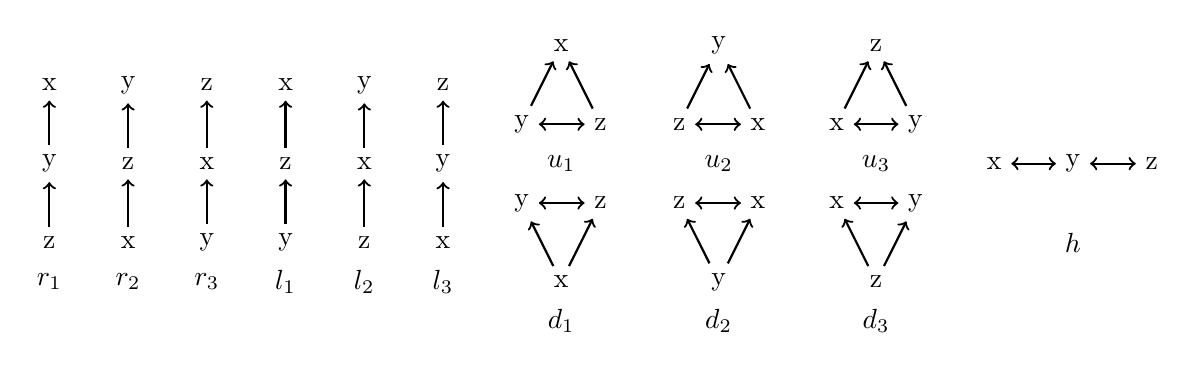
\begin{tikzpicture}
        \node (r1x) at (0,2) {x};  \node (r1y) at (0,1) {y};  \node (r1z) at (0,0) {z};  \node (r1n) at (0,-0.5) {$r_1$};
        \node (r2x) at (1,0) {x};  \node (r2y) at (1,2) {y};  \node (r2z) at (1,1) {z};  \node (r2n) at (1,-0.5) {$r_2$}; 
        \node (r3x) at (2,1) {x};  \node (r3y) at (2,0) {y};  \node (r3z) at (2,2) {z};  \node (r3n) at (2,-0.5) {$r_3$};
        \node (l1x) at (3,2) {x};  \node (l1y) at (3,0) {y};  \node (l1z) at (3,1) {z};  \node (l1n) at (3,-0.5) {$l_1$};
        \node (l2x) at (4,1) {x};  \node (l2y) at (4,2) {y};  \node (l2z) at (4,0) {z};  \node (l2n) at (4,-0.5) {$l_2$};
        \node (l3x) at (5,0) {x};  \node (l3y) at (5,1) {y};  \node (l3z) at (5,2) {z};  \node (l3n) at (5,-0.5) {$l_3$};
        \node (u1x) at (6.5, 2.5) {x};  \node (u1y) at (6.0, 1.5) {y};  \node (u1z) at (7.0, 1.5) {z};  \node (u1n) at (6.5, 1) {$u_1$};
        \node (u2x) at (9.0, 1.5) {x};  \node (u2y) at (8.5, 2.5) {y};  \node (u2z) at (8.0, 1.5) {z};  \node (u2n) at (8.5, 1) {$u_2$};
        \node (u3x) at (10.0,1.5) {x};  \node (u3y) at (11.0,1.5) {y};  \node (u3z) at (10.5,2.5) {z};  \node (u3n) at (10.5,1) {$u_3$};
        \node (d1x) at (6.5,-0.5) {x};  \node (d1y) at (6.0, 0.5) {y};  \node (d1z) at (7.0, 0.5) {z};  \node (d1n) at (6.5, -1) {$d_1$};
        \node (d2x) at (9.0, 0.5) {x};  \node (d2y) at (8.5,-0.5) {y};  \node (d2z) at (8.0, 0.5) {z};  \node (d2n) at (8.5, -1) {$d_2$};
        \node (d3x) at (10.0,0.5) {x};  \node (d3y) at (11.0,0.5) {y};  \node (d3z) at (10.5,-0.5){z};  \node (d3n) at (10.5,-1) {$d_3$};
        \node (hx) at (12,1) {x};  \node (hy) at (13,1) {y};  \node (hz) at (14,1) {z};  \node (hn) at (13,0.0) {$h$};
        \draw [thick,->] (r1z) -- (r1y); \draw [thick,->] (r1y) -- (r1x);
        \draw [thick,->] (r2x) -- (r2z); \draw [thick,->] (r2z) -- (r2y);
        \draw [thick,->] (r3y) -- (r3x); \draw [thick,->] (r3x) -- (r3z);
        \draw [thick,->] (l1y) -- (l1z); \draw [thick,->] (l1z) -- (l1x);
        \draw [thick,->] (l2z) -- (l2x); \draw [thick,->] (l2x) -- (l2y);
        \draw [thick,->] (l3x) -- (l3y); \draw [thick,->] (l3y) -- (l3z);
        \draw [thick,->] (u1y) -- (u1x); \draw [thick,->] (u1z) -- (u1x); \draw [thick,<->] (u1y) -- (u1z);
        \draw [thick,->] (u2z) -- (u2y); \draw [thick,->] (u2x) -- (u2y); \draw [thick,<->] (u2z) -- (u2x);
        \draw [thick,->] (u3x) -- (u3z); \draw [thick,->] (u3y) -- (u3z); \draw [thick,<->] (u3x) -- (u3y);
        \draw [thick,<-] (d1y) -- (d1x); \draw [thick,<-] (d1z) -- (d1x); \draw [thick,<->] (d1y) -- (d1z);
        \draw [thick,<-] (d2z) -- (d2y); \draw [thick,<-] (d2x) -- (d2y); \draw [thick,<->] (d2z) -- (d2x);
        \draw [thick,<-] (d3x) -- (d3z); \draw [thick,<-] (d3y) -- (d3z); \draw [thick,<->] (d3x) -- (d3y);
        \draw [thick,<->] (hx) -- (hy); \draw [thick,<->] (hy) -- (hz);
    \end{tikzpicture}
    \caption{3選択肢の選好}
\end{figure}

二分選好の集合DPの要素である選好の集合は,同率の選択肢が存在する選好のみからなるので,$DP = 2^{\{u_1,u_2,u_3,d_1,d_2,d_3,h\}} - \{\varnothing\}$です.

同調選好の集合EPでは,r,lが0個の要素は$\{u_1,u_2,u_3,d_1,d_2,d_3,h\}$の部分集合全体になります.r,lが1つある場合は以下,
\begin{equation*}
    \begin{array}[h]{c}
        \{r_1,u_1,u_2,d_2,d_3,h\},
        \{r_2,u_2,u_3,d_1,d_3,h\},
        \{r_3,u_1,u_3,d_1,d_2,h\},\\
        \{l_1,u_1,u_3,d_2,d_3,h\},
        \{l_2,u_1,u_2,d_1,d_3,h\},
        \{l_3,u_2,u_3,d_1,d_2,h\}
    \end{array}
\end{equation*}
の6つの各集合の部分集合全体になります.この表記だと$r_1$などr,lを含まない部分集合も含まれますが,そのような集合はr,lが0個の要素としてすでに検出したものと一致するので問題ありません.r,lが2つある場合は,
\begin{equation*}
    \begin{array}[h]{c}
        \{r_1,l_1,u_1,d_2,d_3,h\},
        \{r_1,l_2,u_1,u_2,d_3,h\},
        \{r_2,l_2,d_1,u_2,d_3,h\},\\
        \{r_2,l_3,d_1,u_2,u_3,h\},
        \{r_3,l_1,u_1,d_2,u_3,h\},
        \{r_3,l_3,d_1,d_2,u_3,h\}
    \end{array}
\end{equation*}
の6つの各集合の部分集合全体です.よって$EP$は,
\begin{align*}
EP = & 2^{\{u_1,u_2,u_3,d_1,d_2,d_3,h\}}\\
     & \cup 2^{\{r_1,u_1,u_2,d_2,d_3,h\}}
       \cup 2^{\{r_2,u_2,u_3,d_1,d_3,h\}}
       \cup 2^{\{r_3,u_1,u_3,d_1,d_2,h\}}\\
     & \cup 2^{\{l_1,u_1,u_3,d_2,d_3,h\}}
       \cup 2^{\{l_2,u_1,u_2,d_1,d_3,h\}}
       \cup 2^{\{l_3,u_2,u_3,d_1,d_2,h\}}\\
     & \cup 2^{\{r_1,l_1,u_1,d_2,d_3,h\}}
       \cup 2^{\{r_1,l_2,u_1,u_2,d_3,h\}}
       \cup 2^{\{r_2,l_2,d_1,u_2,d_3,h\}}\\
     & \cup 2^{\{r_2,l_3,d_1,u_2,u_3,h\}}
       \cup 2^{\{r_3,l_1,u_1,d_2,u_3,h\}}
       \cup 2^{\{r_3,l_3,d_1,d_2,u_3,h\}}
       - \{\varnothing\}
\end{align*}
です.

敵対選好の集合$AP$は,r,lが0の要素は先程と同様に$\{u_1,u_2,u_3,d_1,d_2,d_3,h\}$の部分集合全体です.r,lが3つ以上含まれることはありません.r,lが1つまたは2つある時は,
\begin{equation*}
    \{r_1,l_3,u_2,d_2,h\},\{r_2,l_1,u_3,d_3,h\},\{r_3,l_2,u_1,d_1,h\}
\end{equation*}
の各集合の部分集合全体です.よって,$AP$は,
\begin{align*}
AP = & 2^{\{u_1,u_2,u_3,d_1,d_2,d_3,h\}} 
       \cup 2^{\{r_1,l_3,u_2,d_2,h\}} \\
     & \cup 2^{\{r_2,l_1,u_3,d_3,h\}} 
       \cup 2^{\{r_3,l_2,u_1,d_1,h\}}
       - \{\varnothing\}
\end{align*}
です.

極値制限の集合$ER$は,r,lが0,1つの時は$EP$と同じになります.r,lが3つ以上含まれることはありません.r,lが2つのときは
\begin{equation*}
    \begin{array}[h]{c}
        \{r_1,l_1,u_1,d_2,d_3,h\},
        \{r_1,l_2,u_1,u_2,d_3,h\},
        \{r_1,l_3,d_2,u_2,h\},     \\
        \{r_2,l_1,u_3,d_3,h\},
        \{r_2,l_2,d_1,u_2,d_3,h\},
        \{r_2,l_3,d_1,u_2,u_3,h\}, \\
        \{r_3,l_1,u_1,d_2,u_3,h\}.
        \{r_3,l_2,d_1,u_2,u_3,h\},
        \{r_3,l_3,d_1,d_2,u_3,h\}
    \end{array}
\end{equation*}
です.よって$ER$は,
\begin{align*}
ER = & 2^{\{u_1,u_2,u_3,d_1,d_2,d_3,h\}}\\
     & \cup 2^{\{r_1,u_1,u_2,d_2,d_3,h\}}
       \cup 2^{\{r_2,u_2,u_3,d_1,d_3,h\}}
       \cup 2^{\{r_3,u_1,u_3,d_1,d_2,h\}}\\
     & \cup 2^{\{l_1,u_1,u_3,d_2,d_3,h\}}
       \cup 2^{\{l_2,u_1,u_2,d_1,d_3,h\}}
       \cup 2^{\{l_3,u_2,u_3,d_1,d_2,h\}}\\
     & \cup 2^{\{r_1,l_1,u_1,d_2,d_3,h\}}
       \cup 2^{\{r_1,l_2,u_1,u_2,d_3,h\}}
       \cup 2^{\{r_1,l_3,u_2,d_2,h\}}    \\
     & \cup 2^{\{r_2,l_1,u_3,d_3,h\}}
       \cup 2^{\{r_2,l_2,d_1,u_2,d_3,h\}}
       \cup 2^{\{r_2,l_3,d_1,u_2,u_3,h\}}\\
     & \cup 2^{\{r_3,l_1,u_1,d_2,u_3,h\}}
       \cup 2^{\{r_3,l_2,u_1,d_1,h\}}
       \cup 2^{\{r_3,l_3,d_1,d_2,u_3,h\}}
       - \{\varnothing\}
\end{align*}
です.以上より,$DP \cup AP \cup EP$を計算すると$ER$と同じになり,$DP \cup AP \cup EP = ER$です.よって二分選好,敵対選好,同調選好のどれかであることは価値制限を満たすことと同値です.
\end{proof}

図13について考えます.$DP \subset AP$,$DP \subset EP$となることは簡単に確認できます.$|DP|$は,
\begin{equation*}
    |DP| = 2^7 - 1 = 127
\end{equation*}
です.

$AP \cap EP$は,
\begin{align*}
    AP \cap EP = &
        2^{\{u_1,u_2,u_3,d_1,d_2,d_3,h\}} \\
      & \cup 2^{\{r_1,u_2,d_2,h\}} 
        \cup 2^{\{r_2,u_3,d_3,h\}} 
        \cup 2^{\{r_3,u_1,d_1,h\}} \\ 
      & \cup 2^{\{l_1,u_3,d_3,h\}} 
        \cup 2^{\{l_2,u_1,d_1,h\}} 
        \cup 2^{\{l_3,u_2,d_2,h\}} - \{\varnothing\}
\end{align*}
ですが,重複部分がないようにすると,
\begin{align*}
    AP \cap EP = &
        2^{\{u_1,u_2,u_3,d_1,d_2,d_3,h\}} \\
      & \cup (2^{\{r_1,u_2,d_2,h\}} - 2^{\{u_2,d_2,h\}})
        \cup (2^{\{r_2,u_3,d_3,h\}} - 2^{\{u_3,d_3,h\}}) \\
      & \cup (2^{\{r_3,u_1,d_1,h\}} - 2^{\{u_1,d_1,h\}})  
        \cup (2^{\{l_1,u_3,d_3,h\}} - 2^{\{u_3,d_3,h\}}) \\
      & \cup (2^{\{l_2,u_1,d_1,h\}} - 2^{\{u_1,d_1,h\}}) 
        \cup (2^{\{l_3,u_2,d_2,h\}} - 2^{\{u_2,d_2,h\}}) - \{\varnothing\}
\end{align*}
であり,結局,
\begin{equation*}
    |AP \cap EP| = 2^7 + 6 \times (2^4 - 2^3) - 1 = 175 
\end{equation*}
です.同様にして,
\begin{equation*}
    |AP| = 2^7 + 3 \times (2^5 - 2^3) - 1 = 199
\end{equation*}
\begin{equation*}
    |EP| = 2^7 + 6 \times (2^6 - 2^5) + 6 \times (2^6 - 2^5 - 2^5 + 2^4) - 1 = 415
\end{equation*}
となり,図13が書けます.

さて,多数決決定法がどのような時にアロー4条件を見てきたのですが,図13を見ると3選択肢で極値制限を満たす,すなわちその制限の中では個人的選好の自由が保証されるというような選好の組は全体の5\%程度しかありません.

参考文献[3]によると,同率を許さない強順序の選好を各個人がランダムに行った時,3選択肢での多数決決定法で勝者,すなわち,他のどの選択肢に対しても多数となっているような選択肢が現れない確率は図14のようになります.

\begin{figure}[!h]
    \centering
    \begin{tabular}{|cc|cc|} \hline
        人数 & 確率 & 人数 & 確率 \\ \hline 
         1 & 0.0000 & 17 & 0.0827 \\ 
         3 & 0.0556 & 19 & 0.0832 \\ 
         5 & 0.0694 & 21 & 0.0836 \\ 
         7 & 0.0750 & 23 & 0.0840 \\ 
         9 & 0.0780 & 25 & 0.0843 \\ 
        11 & 0.0798 & $\vdots$ & $\vdots$ \\
        13 & 0.0811 & $\infty$ & 0.0877 \\ 
        15 & 0.0820 & & \\ \hline
    \end{tabular}
    \caption{3選択肢で多数決決定法の勝者が現れない確率}
\end{figure}

こうして見ると,3選択肢に限れば,たとえどれだけの人がいても9割以上の確率で決着が付くのです.次に人数を無限にしたままで選択肢の数を増やして行ったものが図15です.

\begin{figure}[!h]
    \centering
    \begin{tabular}{|cc|cc|} \hline
        選択肢 & 確率   & 選択肢 & 確率 \\ \hline
        1      & 0.0000 & 20     & 0.6811 \\
        2      & 0.0000 & 25     & 0.7297 \\
        3      & 0.0877 & 30     & 0.7648 \\
        4      & 0.1755 & 35     & 0.7914 \\
        5      & 0.2513 & 40     & 0.8123 \\
        10     & 0.4887 & 45     & 0.8292 \\
        15     & 0.6087 & & \\ \hline
    \end{tabular}
    \caption{n選択肢で多数決決定法の勝者が現れない確率}
\end{figure}

今度はかなり急激に確率が上昇してしまいます.選択肢が10を超えると半分以上の確率で勝者が決まりません.20にもなると,7割近くで決着が付きません.極値制限を満たしていれば決着はつきますが,決着が付くからと言って極値制限を満たしているわけではないですし,こう見ると極値制限を満たしているという条件はずいぶん個人的選好を制限してしまっているというふうに捉えても良いように思えます.

しかし,極値制限の導入を完全に否定しきることも難しいです.今まで多数決決定法がアロー4条件を満たすための個人的選好の制限について見てきましたが,これは社会の構成員が皆互いにある程度類似した判断をしている時は社会的な決定に決着が付くということだと考えても良いでしょう.こうなると,ある程度の制約を満たしていることが社会で合意を得るために必要な条件だということで,個人が相互配慮をして選好することを社会的な規則として導入するということも,民主的な投票と言える範疇から外れないのではないかというようにも考えられないでしょうか.

我々人間も所詮は動物なのです.我々の社会を個体の集団として捉えると,その社会の維持のために動物的本能として軋轢を生じさせないように意見を変えさせるような社会的圧力を受け入れるというのは,一見民主的ではないように思えても,生態系という観点から見ると自然なことだと言うこともできるでしょう.

しかし,そもそもこの極値制限に道徳的解釈や倫理的正当化を付すことができるでしょうか?もし,それができるような文化であれば,そのような投票方式が採用されるのかもしれませんが,実際には,「運良くこういうパターンの選好になったら,多数決決定法でも循環が起きたりしない」以上の意味合いを持たせられないようにも思えます.

多数決決定法を正当化するには,この個人的選好の自由という条件についてだけ見るのでは苦しいような気もします.他の条件についても考えてみましょう.



\subsection{多数決決定法の強み}

今まで多数決決定法について色々見てきました.実は多数決決定法にしかできないことというのがあって,この節ではそれについて述べたいと思います.

まず,今まで社会的厚生関数や社会的決定関数と言っていたものをもう少し一般化します.

\begin{dfn}[集合的選択規則]
    集合的選択規則とは,n人の個人的選好の弱順序の任意の組$(P_1,\dots,P_n)$に対して,社会的選好の二項関係をただ1つに割り当てる関数関係のことです.
\end{dfn}

社会的厚生関数では社会的選好が弱順序でしたが,集合的選択規則ではその制限はありません.しかし,同じ選択肢同士は少なくとも同程度以上にみなすべきなので,反射性は成り立つものとしてよいでしょう.

\begin{dfn}[決定力]
    集合的選択規則に決定力があるとは,その値域が完全性を持つ二項関係に限定されているということです.
\end{dfn}

集合的選択規則による社会的選好に完全性も求めるということです.社会的厚生関数は推移性を満たす決定力のある集合的選択規則,社会的決定関数は非循環性を満たす決定力のある集合的選択規則であると言えるでしょう.

\begin{lem}
    無関係選択肢からの独立性を満たす任意の決定力がある集合的選択規則の$A$の異なる2選択肢$x,y$に関する社会的選好は,$x,y$に関する個人的選好の関数でなければならない.
\end{lem}

これは無関係選択肢からの独立性の定義より明らかです.

次に集合的選択規則に関する3つの条件を定義します.この3つの条件の定義において,集合的選択規則$f$は,個人的選好のn組$(P^1_1,\dots,p^1_n)$と$(P^2_1,\dots,P^2_n)$をそれぞれ社会的選好$\succeq^1$と$\succeq^2$に写像するものとします.

\begin{dfn}[個人の平等性]
    個人的選好のn組$(P^1_1,\dots,P^1_n)$を並び変えて$(P^2_1,\dots,P^2_n)$としたとき,すべての選択肢$x,y$に対して$x \succeq^1 y \leftrightarrow x \succeq^2 y$を満たすとき,$f$は個人の平等性を満たすと言います.
\end{dfn}

これは,たとえばn組の一番始めの人が独裁者になるというような$f$は個人の平等性を満たさないということです.これは$f$が投票用紙に名前を書かない,誰が投票したかわからないという投票方式だということであり,実質的に1人1票,個人の平等性を意味します.

\begin{dfn}[選択肢の平等性]
    すべての4選択肢$x,y,z,w$に対して,
    \begin{equation*}
        \forall i (x \geq^1_i y \leftrightarrow z \geq^2_i w) \land \forall i (y \geq^1_i x \leftrightarrow w \geq^2_i z)
        \to (x \succeq^1 y \leftrightarrow z \succeq^2 w) \land (y \succeq^2 x \leftrightarrow w \succeq^2 z)
    \end{equation*}
    の時,$f$は選択肢の平等性を満たすと言います.
\end{dfn}

なんだかよくわからない式が出てきました.この式の意味をちょっと考えてみたいと思います.

前件のところを見てください.これは,選択肢$x,y,z,w$を取ってきたときに「選好1でのxとyの関係,選好2でのzとwの関係が同じ時について考えましょう」という意味です.そして,後件を見ると,「xとyの社会的選好1とzとwの社会的選好2も同じになる」とあります.

例えば,今xとzが5票,yとwが3票を獲得したとします.このとき社会的選好1では「xはyより良い」となったのに,2の方では「wのほうがzより良いです」となってしまったのでは,選択肢ごとに1票が与える価値が異なってきてしまいます.この時選択肢の平等性は,「zはwより良い」となるというのを要請します.このように,選択肢の平等性は全く同じ選好状況に対しては全く同じ結論にならなければならないということを要請します.

さらに,選択肢の平等性は選択肢を入れ替えても成り立っていなければなりません.これは,選択肢の名前などではなく,選択肢そのものやその質的なもの,内実に対して評価をして選択をしているということを保証します.

もしも選択肢の平等性がないと,社会的選好に対する信頼性が失われることは容易に想像がつきます.先程の例でzでなくwが社会的に選ばれたらzに投票した人を説得することは難しいでしょう\footnote{ただし,この章の最後でこの条件を否定しにかかりますが.}.

\begin{dfn}[正の反応性]
    すべての2つの選択肢$x,y$に対して,
    \begin{equation*}
        \begin{array}[h]{l}
            [\forall i ((x >^1_i y \to x >^2_i y) \land (x \doteq^1_i y \to x \geq^2_i y)) \land \\
            \exists j ((x \doteq^1_j y \land x >^2_j y) \lor (x <^1_j y \land x \geq^2_j y))
            ] \to (x \succeq^1 y \to x \succ^2 y)
        \end{array}
    \end{equation*}
    の時,$f$は正の反応性を持つと言います.
\end{dfn}

なにがなんなんだっていう感じの式が出てきました.この条件はそんなに大事じゃない(気がする)ので,「そして」から始まる段落まで読み飛ばして頂いても構いません.

$\forall i ((x >^1_i y \to x >^2_i y) \land (x \doteq^1_i y \to x \geq^2_i y))$の意味を考えてみます.これは,任意の個人$i$は,選好1で「xはyより良い」と思ってたら選好2でも「xはyより良い」のままで,選好1で「xとyは同じ」と思っていたら選好2では「xとyは同じ」のままか「xはyより良い」となっているかのどちらかという意味です.つまり,予めxをyより少なくとも同じくらい良いと評価していた人は,xとyの評価をyを良いとする方向には変えないという状況です.

$\exists j ((x \doteq^1_j y \land x >^2_j y) \lor (x <^1_j y \land x \geq^2_j y))$は,ある個人$j$が,選好1で「xとyは同じ」と思っていたら,選好2では「xはyより良い」となる,または選好1で「yはxより良い」と思っていたら,選好2では「xとyは同じ」か「xはyより良い」となります.つまり,少なくとも誰か1人がもともとyをxより少なくとも同程度には良いと考えていたけれど,xに優位になる方に評価を変えたという状況です.

そして,$x \succeq^1 y \to x \succ^2 y$は,社会的選好1と比べて2では,xとyの評価をyが良いとする方向には変化しないとなります.ここから,正の反応性が要請するのは,xを優位としている人は皆xを優位にしたままで,少なくとも1人が選好をxに優位に変化させた時,社会的選好がもともとxとyを同じとしていたならば,社会的な選好もxを優位にする方向に変化するという意味です.

この3つの性質から多数決決定法に関する衝撃的な事実が導かれて行きます.

\begin{lem}
    個人の平等性を満たす集合的選択規則は,非独裁制です.
\end{lem}

独裁制を満たす場合,ある個人の選好が社会的にも反映されますが,その場合,個人を入れ替えた時の社会的選好が変わることから対偶が真なので,明らかです.また,独裁者がいることが個人の平等性と反するということからも明らかだと思います.

この補題は逆が成立しません.たとえ非独裁制でも,「30歳以上は1人2票,30歳未満は1人1票」というような投票方式は個人の平等性を満たしていません.このように,個人の平等性は非独裁制の条件を厳しくしたものだと言えます.

\begin{lem}
    選択肢の平等性を満たす集合的選択規則は,無関係選択肢からの独立性を満たします.
\end{lem}

選択肢の平等性の式の$z,w$に$x,y$を代入すると,無関係選択肢からの独立性の式と同じになります.これもまた逆は成り立ちません.よって,選択肢の平等性は無関係選択肢からの独立性の条件を厳しくしたものだと言えます.

\begin{lem}
    選択肢の平等性と正の反応性を満たす集合的選択規則は,社会の決定性を満たします.
\end{lem}

選択肢の平等性より$\forall i (x \doteq_i y) \to x \simeq y$です\footnote{zにy,wにxを代入します.}.これと,正の反応性より$\exists i (x >_i y) \land \forall i (x \geq_i y) \to x \succ y$なので,結局,社会の決定性$\forall i (x >_i y) \to x \succ y$は当然満たされます.

こう見ると,アロー4条件は案外弱いものだったということに気づいてもらえると思います.

\begin{thm}
    個人的選好の自由,個人の平等性,選択肢の平等性,正の反応性を持つことは,決定力のある集合的選択規則が多数決決定法となるための必要十分条件です.
\end{thm}

多数決決定法は社会的厚生関数ではありません.しかし,反射性と完全性を満たし,アロー4条件を厳しくした上の3つの条件をすべて満たし,かつ個人的選好の自由を保証するような集合的選択規則は多数決決定法しかないのです.

\begin{proof}
必要性は簡単です.多数決決定法が{\bf 決定力のある集合的選択規則の制約下}で個人的選好の自由は,任意の2選択肢$x,y$に対して$x \succeq y$または$x \preceq y$であることから満たされます.個人の平等性,選択肢の平等性を満たすことも明らかです.多数決決定法では,誰かが$x,y$の$x$の方に優位に選好を変えた時,社会的に$y$に優位に傾くことはないので,正の反応性も満たされます.

十分性を示します.補題5.3より,無関係選択肢からの独立性を満たし,補題5.1より,2選択肢$x,y$に関する社会的選好は各個人の$x,y$に関する社会的選好のみによって定まります.また,個人の平等性より,$x,y$に関する社会的選好は「xをyより好むもの」「yをxより好むもの」「xをyと同程度に好むもの」の人数にのみ依存しなければなりません.

選択肢の平等性より,$N(x > y) = N(x < y) \to x \simeq y$です.というのも,$N(x > y) = N(x < y)$を仮定し,$x$と$y$を入れ替えただけで個人の選好が変わっていない個人的選好$>'$で,$N(x \geq y) = N(y \geq' x), N(y \geq x) = N(x \geq' y)$です.

選択肢の平等性で,zにy,wにxを代入すると,$(x \succeq y \leftrightarrow y \succeq' x) \land (y \succeq x \leftrightarrow x \succeq' y)$となります.

$N(x \geq y) = N(y \geq x) = N(x \geq' y)$,同様に$N(y \geq x) = N(y \geq' x)$であり,個人の平等性より,$\succeq$と$\succeq'$は同じ選好にならなければなりません.

よって,$x \succ y$と仮定すると,$x \succ y \to x \succ' y \to y \succ x$となり,矛盾します.$y \succ x$の時も同様にして,結局,$x \simeq y$です.

$N(x > y) = N(x < y) \to x \simeq y$が成り立つことがわかったので,正の反応性より,$N(x > y) \geq N(x < y) \to x \succeq y$です.これは多数決決定法の定義そのものに他なりません.
\end{proof}

アロー4条件をすこし強めて社会的選好の制約を弱めると,多数決決定法のみが条件を満たすのです.多数決決定法は,循環を簡単に起こせるため社会的厚生関数や社会的決定関数にはなりえません.しかし,結果がどうなるかというのを度外視してみれば,我々の日常的な感覚と同じく,公平公正な投票方式と言えるだけでなく,多数決決定法は他の投票方式よりも優れている点が多いと言えるでしょう.


\subsection{社会の決定性と自由主義のパラドックス}

社会の決定性は明らかに受け入れられることのように思われます.全員が賛成しているのだったなら,当然社会的にも認められるべきだというのは,尤もらしいという感じがします.

しかし,社会の決定性を認めると,奇妙なことが起こり得るのです.

\begin{dfn}[自由主義]
    任意の個人$i$は少なくとも1つの異なる選択肢のペア$x,y$に対して決定力を持つ.
\end{dfn}

つまり,自由主義が認められる社会においては,どの個人もある選択肢の組に対して$D_i(x \succ y) \land D_i(x \prec y)$ということです.今後,このことを個人$i$は,$x,y$の社会的選好を決める権利があると言います.

\begin{dfn}[弱い自由主義]
    少なくとも2人のある個人$j,k$は,ある2つの異なる選択肢のペア$x,y$と$z,w$に対してそれぞれ決定力を持つ.
\end{dfn}

これは明らかに自由主義を弱めたものです.

さて,「これが自由主義だ」と言われてもなんのことなのかよくわかりません.2つ例を挙げて説明したいと思います.

\subsubsection*{例1.父と息子の会話(センのパラドックス改)}
ある家庭で父と息子が話をしてるところを想定してください.
\begin{align*}
    息子 & 「お父さん,僕○○大学に行きたいんだよ」 \\
    父   & 「うちは貧乏だから学費は出せないよ」 \\
    息子 & 「でも行きたいんだよ」 \\
    父   & 「大学なんて行ってないで就職しなさい」 \\
    息子 & 「まだ就職はしたくないんだよ」 \\
    父   & 「なんだと?無職になる気か?そんな子に育てた覚えはないぞ」 \\
    息子 & 「でも,就職するぐらいだったら無職の方がマシだね」 \\
    父   & 「なんだと!?それだけは絶対に許さんぞ!!」
\end{align*}

さて,今自由主義と社会の決定性が成立することを仮定しましょう.そして3つの選択肢$x,y,z$を,
\begin{align*}
    就職 : & 息子は就職する \\
    進学 : & 息子は進学する \\
    無職 : & 息子は無職になる
\end{align*}
とします.すると,息子と父の選好は以下のようになります.
\begin{align*}
    父   :& 就職 > 進学 > 無職 \\
    息子 :& 進学 > 無職 > 就職 
\end{align*}
ここで,自由主義の要請について考えます.今,父は息子に学費を出さない自由を持っています.よって,社会的(というか家庭的)にも「$就職 \succ 進学$」が選好されます.また,息子には就職するか無職になるか選択する自由があるはずです.よって,社会的にも「$無職 \succ 就職$」が選好されます.また,父も息子も$進学 > 無職$では共通しているので,社会の決定性より「$進学 \succ 無職$」です.しかし,これでは図17のように循環が起きてしまいます.

ここで,今まで同様「社会的」という言葉を用いてきました.父が学費を出すか,息子が働くか,というのは家庭の問題だというのは,おそらく正しいでしょう.社会的選好や個人の自由というのがこの例に関係あるのかという感じもしますが,ここで言う自由主義は,父・息子が持つ自分の社会的に容認された権利の中での選択は,社会的にも容認されるべきだという立場を取っていることに気をつけてください.

例えば自分が東京に住むか,大阪に住むかを決めるのは自分の権利であり,そのような問題を社会的決定の対象に含めていいのかというのは確かに問題です.しかし,今まで個人的選好をもとに決定を下すことの限界や問題を見てきたわけで,そのような決定の方法を見限らずに,どこまでできるのか,どう理論を構築すればいいのかを考えることは意味があることなのだろうと思います.

\begin{figure}[!h]
    \label{fig:17}
    \centering
    \begin{tikzpicture}
        \node (1) at (1, 1.7) {就職};
        \node (2) at (0, 0) {進学};
        \node (3) at (2, 0) {無職};
        \draw[thick,->] (1) -> (3);
        \draw[thick,->] (3) -> (2);
        \draw[thick,->] (2) -> (1);
    \end{tikzpicture}
    \caption{社会的選好}
\end{figure}

\subsubsection*{例2.新築の屋根の色(ギバードのパラドックス)}
AさんとBさんが二軒並んだ新築の一軒家を購入しました.AさんとBさんは塗装業者に行って屋根を塗ってもらうことにしました.さて,今Aさんは「Bと同じ色は嫌だなあ」と思っていて,Bさんは「Aと同じ色がいいなあ」と思っています.

\begin{align*}
    業者 & 「赤色と緑色ならお安くできます」 \\
    Aさん& 「じゃあそうしよう」\\
    Bさん& 「そうしようそうしよう」\\
    Aさん& 「じゃあ,僕は赤色にしようかな」\\
    Bさん& 「じゃ,私も赤色で」\\
    Aさん& 「え?じゃあ緑色に変えます」\\
    Bさん& 「えー.やっぱ緑色で」\\
    Aさん& 「うーむ.赤色にしますわ……」\\
         &  (以下略)
\end{align*}

と,このように循環が起こってしまいます.なぜこのようなことが起こったのか理由は明らかかと思いますが,一応説明します.まず,社会的な選択肢は,Aの選択する色XとBのそれYを$(X,Y)$とすると,以下の4つ
\begin{equation*}
    (赤,赤),(赤,緑),(緑,赤),(緑,緑)
\end{equation*}
になります.この時,A,Bの個人的選好は,
\begin{align*}
    A : & (赤,緑) \doteq_A (緑,赤) >_A (赤,赤) \doteq_A (緑,緑) \\
    B : & (赤,赤) \doteq_B (緑,緑) >_B (赤,緑) \doteq_B (緑,赤)
\end{align*}
です.そして,Aは$(赤,緑) \succ (緑,緑)$,$(緑,赤) \succ (赤,赤)$とする自由があり,Bは$(赤,赤) \succ (赤,緑)$,$(緑,緑) \succ (緑,赤)$とする自由があります.そのため,社会的選好は図18のようになり,循環してしまいます.

\begin{figure}[!h]
    \centering
    \begin{tikzpicture}
        \node (1) at (0,3) {(赤,赤)};
        \node (2) at (4,3) {(緑,赤)};
        \node (3) at (4,0) {(緑,緑)};
        \node (4) at (0,0) {(赤,緑)};
        \draw[thick,->] (1) -- (2);
        \draw[thick,->] (2) -- (3);
        \draw[thick,->] (3) -- (4);
        \draw[thick,->] (4) -- (1);
        \node (5) at (2,3.3) {Aの自由};
        \node (6) at (5,1.5) {Bの自由};
        \node (7) at (2,-0.4) {Aの自由};
        \node (8) at (-1,1.5) {Bの自由};
    \end{tikzpicture}
    \caption{社会的選好}
\end{figure}

この例では社会の決定性は全く関係しません.社会の決定性だけが自由主義の下で循環を起こす要因ではないということです.しかし,筆者の力不足と調査不足のため,このような場合への考察はここではしません.誰か教えてください.

さて,例1,2のように,個人の自由というものを社会に容認させると,社会的選好の循環が起こりえます.これを自由主義のパラドックス,あるいはリベラル・パラドックスと言います.

\begin{thm}[センの不可能性定理]
    弱い自由主義,個人的選好の自由,社会の決定性を同時に満たす社会的決定関数は存在しません.
\end{thm}

\begin{proof}
個人$j,k$,選択肢$x,y,z,w$で,$j$は$x,y$の社会的選好を決める権利があり,$k$は$z,w$の社会的選好を決める権利があるとします.

今,この2人に決める権利のある選択肢に共通の要素があるとします.2つの要素が共通する時はお互い相反する選好をしうるので,明らかに個人的選好の自由を満たしません.1つの要素が共通するときについて考えます.例えば$x = z$とします.

個人的選好の自由より,どのような個人の選好に対しても社会的選好が1つ定まります.そこで,$x >_j y$,$w > _k x$,$\forall i (y >_i w)$と仮定します.この時,$j$の権利より,$x \succ y$.また,$k$の権利より$w \succ x$.そして,社会の決定性より$y \succ w$です.しかし,これは$x \succ y \succ w$となり,循環を生みます.このため,非循環性を満たしません.

次に,共通する選択肢がないときを考えます.$x >_j y$,$z >_k w$,$\forall i (w >_i \land y >_i z)$と仮定します.この時,$j$の権利より$x \succ y$.$k$の権利より$z \succ w$.社会の決定性より$w \succ x,y \succ z$.よって,$x \succ y \succ z \succ w \succ x$となり,非循環性を満たしません.
\end{proof}

さて,ここまで見てきた通り,今まで社会的選好が依るべきとした条件である社会の決定性は,自由主義と相反するものだということがわかりました.そこで,自由主義か社会の決定性のどちらかを制限することを考えたいです.しかし,自由主義を制限することを考えると,「具体的にどの個人のどの権利を制限するか」という問題になってしまいます.まずは社会の決定性がいかに自由主義と矛盾を生じるか考えます.


\subsection{パレート伝染病}
社会の決定性$\forall i (x >_i y) \to x \succ y$の持つ問題は何なのでしょうか.社会の決定性を我々が「民主制に不可欠な」「自然な条件」と認識するのは,その「全員一致の判断は社会的に反映されるべきだ」という側面だけを見ているからだと言えます.社会の決定性は全員の選好の一致が起きている時に限り,無関係選択肢からの独立性,すなわち,$x$と$y$の社会的選好はその個人的選好のみから成り立つとする側面を持ちます.この無関係選択肢からの独立性を弱めたような条件が奇妙な事態を引き起こすのだと考えられます.

具体的にどのような問題が起こるのか考えます.自由主義より,ある個人$k$はある選択肢のペア$x,y$に対する決定力を持つものとします.すなわち$D_k(x\succ y) \land D_k(y \succ x)$.今,選択肢$x,y,z,w$に対して,個人の選好を図19のように,$x >_i y, z >_i w, \forall k (z >_k x), \forall k (y >_k w)$とします.

\begin{figure}[!h]
    \centering
    \begin{tabular}[!h]{|c|c|c|c|} \hline
        & i & その他 & 社会 \\ \hline
        x,y & $x > y$ &    ?    & $x \succ y$ \\ \hline
        y,w & $y > w$ & $y > w$ & $y \succ w$ \\ \hline
        z,x & $z > x$ & $z > z$ & $z \succ x$ \\ \hline
        z,w & $z > w$ &    ?    & $z \succ w$ \\\hline
    \end{tabular}
    \caption{選好}
\end{figure}

社会的選好は図19のようになりますが,表をよく見ると,個人$i$が選択肢のペア$z,w$にも決定力を持ってしまっています.これは,選択肢$y,w$,$z,x$における社会の決定性によるものです.

\begin{figure}[!h]
    \centering
    \begin{tikzpicture}
        \node (1) at (-1, 1) {x};
        \node (2) at ( 1, 1) {y};
        \node (3) at (-1,-1) {z};
        \node (4) at ( 1,-1) {w};
        \draw[thick, ->] (2) -- (1);
        \draw[thick, ->] (1) -- (3);
        \draw[thick, ->] (4) -- (2);
        \draw[ultra thick, ->] (4) -- (3);
        \node (5) at (0, 1.4) {$i$の権利};
        \node (6) at (0,-1.4) {伝染};
        \node (7) at ( 2.2,0) {全員一致};
        \node (8) at (-2.2,0) {全員一致};
    \end{tikzpicture}
    \caption{社会的選好の波及}
\end{figure}

ここで,例えば$z$が「個人$j$\footnote{iではないことに注意してください.}は一週間Twitterでヒシュカリヤナ語縛りをする」,$w$が「個人$j$は一週間Twitterでカシュヤナ語縛りをする」だとした場合,たとえ個人$j$が$w > z$と選好していても$z \succ w$となり,社会の決定性が自由主義を侵害する結果になってしまいます.このように社会の決定性(パレート最適性)と社会的選好が伝染し,個人の権利を侵害することをパレート伝染病と言います.

\subsubsection*{センの解決法}
このような自由主義のパラドックスやパレート伝染病を解決する方法の1つを紹介します.これはセンによるものなので,センの解決法と呼ぶことにします.

まず,センの解決法では,個人的選好を隠すことを許します.例えば,「実は人には言えないこういう趣味がある」などのプライベートなことを社会的に表明せずに隠しておいても良いということです.社会全体で選好が一致しても,誰か一人が選好を隠せば社会の決定性は行使されません.このような意見の保留を許す時,他人の権利が侵害されないように誰かが自分の意見を隠すことでパレート伝染病を防ぐことができます.もっと言えば,一つの社会には「他人の権利を侵害しないように自分の選好を隠す」良心的で自由主義者な個人が一人でも存在するならば,各個人が決定力を行使しても社会の決定性と矛盾しないような決定方式が存在し得るということです.今後,このような個人のことを良心的自由主義者と呼ぶことにします.

先程の「父と息子の会話」の例にこの方法を適用してみましょう.仮に父を良心的自由主義者とします.父は「就職$\succ$進学」とする決定力がありますが,これは社会的循環を発生させ,息子の「無職$\succ$就職」の権利を侵害します.そのため,父は「就職$\succ$進学」の表明を取りやめ,結局社会的には「進学$\succ$無職$\succ$就職」となります.息子が良心的自由主義者の時も同様にして,「就職$\succ$進学$\succ$無職」となります.まあ,「良心的自由主義者」などと言っていますが,この場合は息子が諦めて就職するという感じなのでしょうが.また,ここで誰が良心的自由主義者となるのかという問題も生じますが,それ以上は社会的倫理などの領域になるかと思われますし,考察を止めたいと思います.

今までの議論で見てきたように,社会の決定性には選択肢の中に含まれる個人の権利を侵害することがあります.選択肢と言って我々が普通イメージするのは,例えば「本を一冊選んでください」という状況での,「資本論」「国富論」「幸福論」などのようなものです.しかし,選択肢が対象とするものは単なるモノだけではなく,個人の権利や社会的に意味を持つ個人の選択なども含まれて来てしまいますし,そのような選択肢が存在しうることについても考慮しなければなりません.

このような社会的な選択は,単に選択肢間の順位付けをするだけでなく,その決定における倫理性というものをも規定することができます.これに関しては詳しいことは専門的な図書を当たるなどして調べていただきたいです.社会の決定性が引き起こしうる問題点について理解し,後述する架空世界の投票方式の考察でより深い理解を得るための参考にしていただければよいかと思われます.


\subsection{開かれた社会的決定}

今,客がウェイターに注文を取っているところを想定してください.以下のように会話しているとします.
\begin{align*}
    ウェイター &  「本日はトンカツとステーキのみとなっております」 \\
    客         &  「じゃあ,ステーキにするよ」 \\
    ウェイター &  「あっ.伊勢海老のグリルもお出しできますが」 \\
    客         &  「おっと.えー,うーん.じゃあ,やっぱりトンカツにするよ」 
\end{align*}
さて,今このお客さんにとって集合$\{トンカツ,ステーキ\}$の最良要素はステーキです.しかし,集合$\{トンカツ,ステーキ,伊勢海老のグリル\}$の最良要素はトンカツとなってしまいます.伊勢海老のグリルという新しい選択肢が増えたことで,すでに決めた選好が変わっているのですが,そのような変化は一見不自然なように思えないでしょうか\footnote{もちろん,客が全く合理性に欠く判断をしたとは断定できませんが.この客の心理を合理的に説明する方法を考えてみるのも面白いかもしれません.}.

無関係選択肢からの独立性が要求していたのは,選択肢の集合の任意の部分集合での社会的選好が変化してはならないという条件でした.上の例のようなことが社会的に起こってはならないということです.ここで,無関係選択肢からの独立性を厳しくした条件である選択肢の平等性を仮定した時に社会的厚生関数が引き起こす奇妙な事態について説明したいと思います.

\subsubsection*{ハンソンの定理}
\begin{thm}[ハンソンの定理]
    個人的選好の自由,個人の平等性,選択肢の平等性を満たす社会的構成関数は,任意の選択肢を同順位としなければなりません.
\end{thm}

誰がなんと言おうと,すべての選択肢が同率1位となってしまいます.そんなこと,あるんでしょうかという感じです.

\begin{proof}
個人の平等性と選択肢の平等性を満たす社会的厚生関数で,2選択肢$x,y$に対して図21のような個人的選好を考えます.このとき,個人の数は偶数人であることを仮定します.社会全体は2n人とし,その内n人を個人の集合A,残りのn人を集合Bとします.
\begin{figure}[!h]
    \centering
    \begin{tabular}[!h]{|c|c|c|c|} \hline
         & A & B & 社会 \\ \hline
        x,y & $x > y$ & $x < y$ & ? \\ \hline
    \end{tabular}
    \caption{個人的選好} 
\end{figure}
さて,今個人の平等性が満たされているので,集合Aの人と集合Bの人をすべて入れ替えても社会的選好は変わりません.つまり,図22のようになります.
\begin{figure}[!h]
    \centering
    \begin{tabular}[!h]{|c|c|c|c|} \hline
         & A & B & 社会 \\ \hline
        x,y & $x < y$ & $x > y$ & ? \\ \hline
    \end{tabular}
    \caption{個人的選好} 
\end{figure}
さらに,選択肢の平等性より,選択肢$x,y$を入れ替えても結果は同じです.つまり,図23のようになります.
\begin{figure}[!h]
    \centering
    \begin{tabular}[!h]{|c|c|c|c|} \hline
         & A & B & 社会 \\ \hline
        y,x & $y > x$ & $y < x$ & (?のx,yを入れ替えたもの) \\ \hline
    \end{tabular}
    \caption{個人的選好} 
\end{figure}

もし,?が$x \succ y$だと仮定すると,図22と図23で同じ個人的選好から異なる社会的選好が定まることになり矛盾します.$x \prec y$も同様です.社会的厚生関数の社会的選好は完全性を満たしているので,$x \simeq y$ということになります.

以上より,個人・選択肢の平等性が満たされ,偶数人で意見が半数ずつ対立すれば,社会的選好は2選択肢を等価とすることがわかります.これは別に奇妙でも何でもなく,普通に受け入れられる事実です.

さて,次に3選択肢$x,y,z$に関して,個人的選好が図24のようになっているとします.
\begin{figure}[!h]
    \centering
    \begin{tabular}[!h]{|c|c|c|c|} \hline
         & A & B & 社会 \\ \hline
        x,y & $x > y$ & $x < y$ & $x \simeq y$ \\ \hline
        y,z & $y < z$ & $y > z$ & $y \simeq z$ \\ \hline
        z,x & $z > x$ & $z > x$ & $z \simeq x$ \\ \hline
    \end{tabular}
    \caption{個人的選好}
\end{figure}
$x,y$,$y,z$間では半数ずつ対立しているので社会的選好はそれらを等価とします.さらに社会的選好の推移性より$z \simeq x$です.選択肢の平等性より,無関係選択肢からの独立性が言えるので,結局,2選択肢間で全員が同じ選好をした時は社会的にその2選択肢は等価とされることがわかりました.

そうすると,結局図25のような場合を考えれば,推移性によって選択肢が同順位であることが波及し,どのような個人的選好に対しても社会的に等価としなければならないことがわかります.
\begin{figure}[!h]
    \centering
    \begin{tabular}[!h]{|c|c|c|c|} \hline
         & A & B & 社会 \\ \hline
        x,y &    ?    &    ?    & $x \simeq y$ \\ \hline
        y,z & $y > z$ & $y > z$ & $y \simeq z$ \\ \hline
        z,x & $z > x$ & $z > x$ & $z \simeq x$ \\ \hline
    \end{tabular}
    \caption{個人的選好}
\end{figure}

次に社会が奇数人である時を考えます.図26のような場合を考えます.Aがn人,Bが{\bf n-1}人とします.
\begin{figure}[!h]
    \centering
    \begin{tabular}[!h]{|c|c|c|c|c|c|} \hline
         & i & j & A & B & 社会 \\ \hline
        x,y & $x > y$ & $x < y$ & $x > y$ & $x < y$ & $?_0$ \\ \hline
        y,z & $y < z$ & $y > z$ & $y > z$ & $y < z$ & $?_1$ \\ \hline
        z,x & $z > x$ & $z < x$ & $z < x$ & $z > x$ & $?_2$ \\ \hline
    \end{tabular}
    \caption{個人的選好}
\end{figure}
個人の平等性より,$?_0$,$?_1$,$?_2$は同じとなります.しかし,$?_0$が$x \succ y$の時,$?_1$が$y \succ z$となり,推移性より$?_2$は$z \prec x$となり矛盾します.$?_0$は$x \prec y$ともなりえず,$x \simeq y$です.同様にして$y \simeq z$,$z \simeq x$です.ここから,n人とn+1人が対立する場合,社会的に等価とみなすことになります.

次に,Aがn+1人,Bがn人であるとします.図27のような場合を考えます.
\begin{figure}[!h]
    \centering
    \begin{tabular}[!h]{|c|c|c|c|c|} \hline
         & A & B & 社会 \\ \hline
        x,y &    ?    &    ?    & $x \simeq y$ \\ \hline
        y,z & $y > z$ & $y < z$ & $y \simeq z$ \\ \hline
        z,x & $z < x$ & $z < x$ & $z \simeq x$ \\ \hline
    \end{tabular}
    \caption{個人的選好}
\end{figure}
n+1人とn人が対立する場合社会的に等価になることと推移性より,x,yに関するどのような個人的選好に対しても,x,yは社会的に等価となります.

以上より,個人と選択肢の平等性を満たす社会的厚生関数は,すべての選択肢を社会的に同順位としなければなりません.
\end{proof}

公正な投票方式として,個人の平等性,選択肢の平等性,社会的選好の推移性は当然満たされるべきだと考えるのは自然なことに思えます.しかし,どのような投票方式も個人の平等性,選択肢の平等性,社会的な推移性を要求するとすべての選択肢を同順位とせざるを得ないという結果が導かれてしまいました.

民主的な社会では当然個人の平等性は満たされているべきです.つまり,現実の投票方式では選択肢の平等性か推移性のどちらかが犠牲になっているということです.しかし,普通我々が行う投票方式は皆社会的な推移性を満たしています\footnote{推移性を満たしていない場合,選挙結果が定まらないような事態が起き得,何も決められないのですが,それでは投票を行う意味がないです.}.つまり,我々は選挙方式の中で選択肢の平等性を完全に満たすことはできません.

例えば,我々が国政選挙などで行っている単記投票方式では投票結果が推移性を満たしています.というのも,投票結果に循環は起こりえないからです.よって,選択肢の平等性を満たしていないということになってしまいます.

これは,単記投票では戦略的投票を許してしまうということです.無関係選択肢からの独立性を満たさないと戦略的投票が起きうるということをボルダ得点法の説明の時に述べました.選択肢の平等性を満たしていないからと言って,必ずしも戦略的投票が起きるとは言えませんが,単記投票では起きてしまいます.例えば,選択肢A,B,Cから単記投票で選ぶ時,「AさんとBさんは大きな政党から推薦をもらっているけど,Cさんはもらっていないから当選の見込みはないだろう.本当は考えとしてはCさんが自分に最も近いが,Aさんには当選してほしくないので,やむを得ずBさんに投票しよう」というような投票行動は自然なものとなってしまいます.

5.3節で選択肢の平等性が投票の信頼性を保証するという旨のことを言いました.しかし,おそらく我々は国政選挙などで各党の政策マニフェストを見て投票する時に,マニフェストの党名を隠して読むか,隠さず読んで判断するかで結果が変わってくるのではないかと思います\footnote{比例代表制の選挙の前日に,例えば突然自民党と共産党の名前が入れ替わったらもともと共産党だった方の政党が勝つと思いませんか?}.5.3節で述べたのはこの条件の「選択肢の名前にかかわらず平等」という点のみだけで,「選択肢の名前を入れ替えても平等」という点のみまで保証することは少し厳しそうです.

\subsubsection*{開かれた社会的決定}
ハンソンの定理から推移性を満たす投票方式は選択肢の平等性を満たしていないことがわかります.アロー4条件から無関係選択肢からの独立性を除けば選択肢の平等性を満たしていないことがことさらに問題にはなりません.しかし,無関係選択肢からの独立性を満たしていないということは,2つの選択肢に関する社会的決定を下すためには,その2つの選択肢以外の選択肢の間の選好関係についても知っていなければならないということを意味します.極端な言い方をすれば,「りんご」と「みかん」の選好を決めるときに,「90式戦車」と「10式戦車」の選好についても考慮しなければならないということです.さすがにそんな馬鹿げたことが問題となる投票はないだろうとは言えるのでしょうが,決定というのは常に暫定的なもので,新たな選択肢が追加されたり,既存の選択肢が削除されたりした時に,すでに決めていた選好が変わることは認めてもいいのかもしれません.一度「りんごはみかんより良い」と決めたらそれが永久に覆らないというのは,むしろ不自然にも思えます.

そこで,「開かれた社会的決定」というものを考えます.

\begin{dfn}
    開かれた社会的決定とは,すでに暫定的に限定された選択肢の集合に,新しい選択肢が追加されたり,あるいはすでにある選択肢が除外されたりした時に,すでに決まっている個人的選好に全く変化がないとしても,すでに決まっているどのような社会的選好も変更されうる可能性があることをすべての個人が了承した上で行われる社会的決定のことです.
\end{dfn}

既存の選択肢だったA党が選挙直前に分裂してB党とC党になったりすると,もともとA党が勝ちそうだったのに,B党もC党も選挙で負けてしまうというように選択肢の消失や追加が社会的選好に影響を与えることをみなさんちゃんと理解してどのように投票するか決めてくださいということです.

それがどうした,という感じもあります.しかし,ハンソンの定理から社会的選好が推移性を満たすなら選択肢の平等性は保証されず,社会的決定は開かれたものであるべきだということが言えます.ハンソンの定理によって,開かれていることを社会に課すことの是非を検討する道理が生まれるのです.

開かれた社会であるべきという態度は言い換えると,単記投票のように個人の細かい選好が見えにくい投票方式では,無関係選択肢からの影響が見えにくいため,各個人が各選択肢をどのような順位で選好するかということも社会的決定に生かそうというものです.これはボルダ得点法を正当化するものです

ボルダ得点法の欠陥はすでに見たとおりです.結局ボルダ得点法は良いのか悪いのかどっちなんだという感じですが,ここで言いたいのは,{\bf 別に無関係選択肢からの独立性を満たしてないからと言って,そんなに深刻な問題ではないですよ}という,3章の伏線の回収と,{\bf 多数決はどうあがいても推移性か平等性のどちらかを失う不完全なものなのですよ}ということです.ボルダ得点法が良いか悪いかはよくわかりません\footnote{利点,欠点というような個性はそれぞれありますが.}.


\subsection{結局}
さて,今までアロー4条件が妥当かについて議論してきました.正直,議論は不十分極まりないという感じですが,どの条件をどこまで破ってもいいのかという点に着目しながら決定方式を議論できると言えなくはない程度のことはしたと思っています.

少し5章全体をまとめたいと思います.そもそも,社会的厚生関数の前提がダメなのではないかということで,推移性を非循環性まで緩めてあげてみると,アロー4条件を満たし得ることを示しました.しかし,あまり良い社会的決定ができる方法にはなりませんでした.

次に具体的にアロー4条件を緩めて検討しました.個人的選好の自由を制限すると社会的選好の推移性は保たることを示しました.しかし,社会的厚生関数となるために必要十分な制限である価値制限を満たすことをどう捉えるかについては,私の力不足ではありますがよくわかりませんし,制限が妥当なものとも言えませんでした.逆に,個人的選好を制限せず,社会的に反射性と完全性だけを満たしていれば良いとすれば,多数決決定法はアロー4条件を厳しくした条件もクリアするかなり優秀な方式と言えることもわかりました.

社会の決定性は場合によっては個人の権利を侵害しうるということを指摘しました.この発想から,社会的決定に倫理性という概念を持ち込むことができることも少し述べました.

無関係選択肢の独立性は,社会が開かれたものであるべきだとするハンソンの定理の要請から,別にそんなに重要な条件でもないと捉えることもできました,単記投票やボルタ得点法などは戦略的投票が可能になってしまいますが,そのようなことを各個人が前提とした社会的決定であれば民主的と言えなくもありません.

非独裁制についてはあまり詳しく述べませんでしたが,それは個人の平等性という条件に含まれるということは見ました.個人の平等性は「一人一票」のように,各個人が投票に関しては同じ権利を持つという条件なので,そう考えると非独裁制はあまり疑う余地がないように個人的には思います\footnote{実際どうなのかは詳しい人教えてください.}.

さて,次に架空世界での投票方式について考えていきたいと思います.


\section{架空世界における社会的決定について考える}
架空世界での社会的決定方式を考えなければいけないというのは,そもそもどういう状況なのでしょうか.例えば,創作の過程で架空世界を作ることになったとき,その世界にある王朝や国家などの共同体が,例え民主的な制度を持っていたとしても,独裁的なものだとしても,聖人君子がなんか話し合って決めごとをしているとしても,なんらかの社会的決定法があると考えるのが妥当です.そこで,どのような手法で権力者や主権者が社会的な決定を下せばいいのかという問題が生じ得ます.それも,単に独裁的に決めればいいわけではなく,合理的で人々の反感を買わないような方法でないと謀反を起こされたり,革命されちゃったりするかもしれませんし,どうすればいいのかと悩むこともあるかもしれません.

もともと,この文書を書き始めたのはそのような異世界においてどのような意思決定法が生まれてくるのだろうという疑問がきっかけでした.私自身も架空世界創作をしたことがあり\footnote{現在もしていますが.},政治レベルでの社会的決定をどうすればいいのかというのは,いまいちちゃんとした理由もなく封建制を導入したり,議会制を導入したりとしていました.

しかし,社会的決定理論の存在を知り,もしかしたらこれで架空世界の意思決定について色々と考察できるのではと考えて調べたりしました.といっても,考察にかけた時間はせいぜい二ケ月ぐらいしかないですし,具体的にどのように制度が出来上がっていくか,正当化されていくかなどと言えるほどの理解には至れませんでした.しかし,歴史的に制度が形成されていく理由を合理的に記述したりするのには役に立つ程度の知識を得ることができたとは思っています.

「投票」というと,議員選挙がイメージされるかもしれません.しかし,政治レベルに限ったとしても,法案の評決は投票ですし,最高裁の判決も投票とは言えないまでも,社会的決定の一種と言えるでしょう.つまり,社会の様々な決定プロセスへと応用が可能です.まずは実際の社会でどのような問題が起こるのかその実例について少し紹介した後に,{\bf 結局,多数決は何をしてもダメ}という本質に迫りたいと思います.

\subsubsection*{18世紀フランス科学アカデミーでの論争}
18世紀,フランス科学アカデミーという学術団体では,その会員を決めるのに単記投票方式を用いていたそうです.しかし,自身も会員だったボルダは単記投票方式には問題があるということを指摘しました.

単記投票にはどのような問題があるのでしょうか.選択肢x,y,zに対して,7人の個人$a\sim g$が図28のように選好しているとします.
\begin{figure}[!h]
    \centering
    \begin{tabular}[!h]{|c|c|c|c|c|c|c|c|} \hline
         & a & b & c & d & e & f & g \\ \hline
        1 & x & x & x & y & y & z & z \\ \hline
        2 & y & y & y & z & z & y & y \\ \hline
        3 & z & z & z & x & x & x & x \\ \hline
    \end{tabular}
    \caption{個人的選好}
\end{figure}
この時,単記投票を取ると,xが最も多く得点します.ここで,逆に最も悪いと思う選択肢はどれかと聞くと,またxが最も多く得点してしまいます.つまり,単記投票ではこの7人が最良と選択する要素と最悪と選択する要素が同じだという結果を導いてしまいます.すべての個人の選好が反転した時に社会的選好が反転前と同一であってはならないとする条件を双対性と言います.この例から単記投票は双対性を満たしていないことがわかります.

ボルダはこのような単記投票の欠陥を指摘し,1784年科学アカデミーの会員の決定方式はボルダ得点法へと変わりました.しかし,3章で説明した通り,ボルダ得点法には戦略的に結果を操作できるという欠陥があります.1800年,ナポレオン・ボナパルトによってそのことを指摘された\footnote{この欠陥を最初に指摘したのはおそらくラプラスで,ナポレオンは二番煎じです.}科学アカデミーはボルダ得点法をやめ,信任投票で会員を決めるようになったそうです.  

\subsubsection*{1955年米上院,道路建設に関する法案を巡る争い\footnote{
    この話は参考文献[1]によるが,その出典はR.Farquharson "Theory of Voting" (1969)らしいです.しかし,原著を閲覧することができず,ネットで検索してもそれらしい情報が見つからないので,信憑性に疑問はあります.誰か情報あればください.架空世界創作の参考になるかが至上命題なので掲載しました.
}}
1955年,米上院で過半を取る民主党は新国道建設法案を上院に提出しました.この時,法案には労働者に公正な賃金を払うとするデービスベーコン法を適用させる一文が盛り込まれていました.これに対して,南部出身の民主党議員からは,北部出身の民主党員による南部への干渉だとの批判が起こりました.南部民主党はデービスベーコン法に関する部分を削除した修正案を提出します.他方,共和党は新法案の撤回を求めました.原案のままでは南部民主党と共和党が反対します.修正案では北部民主党と共和党が反対します.しかし,廃案にするのは民主党の方針に合いません.困りました.

北部共和党はなんとしても法案を通過させたい.南部側はデービスベーコン法の適用だけは何がなんとしても避けたい.他方,実は共和党側は原案と修正案なら原案の方が良いと考えていたのです\footnote{なんでそうなるのかよくわかりませんが,デービスベーコン法の提出者が共和党の人だからなのかなあなどと思いました.誰か教えてください.}.つまり,各陣営の個人的選好は次のようになります.
\begin{align*}
    北部民主党 :&  原案 > 修正案 > 廃案 \\
    南部民主党 :&  修正案 > 廃案 > 原案 \\
    共和党     :&  廃案 > 原案 > 修正案
\end{align*}
よく見ると,最初の昼ご飯の例と同じです.すなわち,投票のパラドックスが生じます.

そこで,民主党の上院議員で党首だったリンドン・ジョンソンと同じく民主党の上院議員アルバート・ゴア・シニアは考えました.実はこの二人,南部出身の民主党員でした.ジョンソンとゴアはどうにかして修正案を通したいと思っていました.ジョンソンの提案で上院はまず,「原案を採択するか,修正や廃案の協議に持ち込むか」で評決を取りました.南部の民主党員と共和党員の反対で協議に入ることになりました.次に修正案か廃案かで評決を取ると,上院で過半数を取っていた民主党員が賛成したため,なんと修正案が通ってしまいました.

これは最初の昼ご飯の例で言うところの,nymwaくんの独断でラーメンを食べることに決定するのと同じです.社会的に選ばれてほしい選択肢の評決を最後に持ってくるのがポイントです.しかし,立法府たる議会でこんな独裁的な議会運営が許されてしまうというのは驚きです\footnote{誰か架空世界創作のネタで使ってください.}.

とまあ,現実でも社会的決定の困難さのせいで様々なパラドックスが生じてしまします.これが民主的な意思決定なのかというのは甚だ疑問です.一体どうすれば民主的と言えるのでしょうか.

\subsection{多数決と民主制は無関係}
先程上げた例ではいずれも単記投票方式が問題の根源となっていることがわかると思います.今までの議論からわかるように,我々が多数決として普段用いているその方式は,欠陥だらけのものだと言えます.特に単記投票では,個人的選好を完全に反映させることができない,つまり死票が多いですし,選択肢をいじれば戦略的に結果を操作でき得ます.それを改善しようとすると,個人的選好の自由を制限したり,社会的選好が循環したりすることを許さなければなりません.

じゃあ,多数決なんかやめようと,もっと根本から逆転の発想でなんとかならないか,とも思えてきます.しかし,社会の全個人の意見を聞いて社会全体の幸福度を最大限にしたり,社会全員が納得したりするような社会的決定を行うことは,その手間の多さや社会の複雑さから考えるとほとんど困難だと言えるでしょう.社会はどうしても個人的選好を入力とした関数としての社会的意思決定を執り行うことになります.そして,そのためにはどこかで社会的決定のルールを決めておかなければ混乱が生まれるだけです.安定的な社会的決定を持続的に行うためには,どこかでルールを決めそのルールにのっとって決めた社会的選好を社会が御神託として受け入れる必要があります.その御神託が奇妙で受け入れ難いものにならないようにしなくてはなりません.しかし,どうしても完璧な御神託を生み出す方式は存在しないというのがアローの不可能性定理ですし,アロー4条件を緩めてみてもいまいち良い妥協点が見つかるわけでもありませんでした.

世の中には様々な投票方式があるらしいです.それぞれがそれなりに利点・欠点を持っています.社会がどの投票方式を選択するかは,それぞれの方法の利点・欠点に依存すると考えられます.それぞれの社会が時代の要請に答えその時々に合う方法を選択して行くと考えられます.例えば,日本では55年体制の崩壊を受け1994年に衆議院議員の選挙制度が中選挙区制から小選挙区比例代表並立制へと変わりました.中選挙区では選挙にお金がかかりますし,リクルート事件などの汚職,政治腐敗などの根絶を求めた政治改革への動きが選挙制度改革の原動力となったそうです.\footnote{ただし,これは比例代表制へと向かう世界の流れと逆行するものだという批判があったり,そもそも導入した側も不本意だったみたいです.\footnotemark}.\footnotetext{http://diamond.jp/articles/-/14406}

それぞれの投票方式には個性というか,良し悪しがあります\footnote{例えばボルダ投票では全員が正直者であるときに合理的とみなせます.}.架空世界における投票方式を考えるということは,その世界での社会の状況や合理性の論理を正当化する投票方式を考えるということなのかもしれまん.ちょっと具体的に見ていきましょう.

\subsection{そうだ,多数決しよう}
多数決は個人の平等性を満たしています.さすがに個人の平等性は満たされるべきですし,多数決に限って比較していきます.

\subsubsection*{単記投票の問題まとめ}
単記投票と今まで漠然と言ってきたが,実は単記投票にもいろいろあります.今までは一回投票してもらって,一番票数が多いものが選ばれるという,いわゆる単純多数決のみを指していましたが,決選投票を行うなど様々な改良を加えたものもあります.

単純多数決には双対性がないことは今まで見たとおりです.また,選択肢xが選ばれたとしても,多くの人がxを支持しているとも言えません.そもそも半数近くの人が投票を棄権していることも考えられますし,先に見たように戦略的投票可能性の問題もあるからです.実はxを最も良いと思っているけど,xが圧勝しそうなのでバランスを取るべきだと考えて異なる選択肢yに投票するというような投票行動なども考えられます.

また,上位二人以上を選出するいわゆる大選挙区制の場合,例えば一選挙区で二人選ぶとして同率二位が発生した場合にどちらが当選するかを公平に選ぶのは難しそうです.この場合,最終的にはくじ引きで決めることになるでしょうが,それが公平と言えるかは怪しいです.決選投票やオーストラリアで行われているような選好投票をすればこの問題自体は解決されます\footnote{ただし別の問題が発生したりするので社会的決定は難しいです.}.

\subsubsection*{多数決決定法の限界まとめ}
多数決決定法は個人と選択肢の平等性を満たすという点に限れば優れた決定方式です.しかし,アローの不可能性定理,ハンソンの定理のいずれからもわかるように社会的選好が必ずしも推移性を保つものになるとは限らないことは今まで見てきたとおりです.

多数決決定法では個人の選好を制限すれば社会的な推移性を満たすことは5章で見たとおりです.実は,個人の数が奇数のとき\footnote{単峰型投票,タブー型投票など.}や,社会に推移性ではなく非循環性を要請したときはより緩い制限\footnote{価値制限,限定的同意など.}ですむのですが,いずれにせよその制限というのが結構厳しくて,個人の選好をかなり制限するものになってしまいます.

\subsubsection*{決選投票方式}
単純多数決では過半数の得票を得ていない選択肢も一位として選ばれ得ます.過半数の信任を得られない選択肢を社会的に選ぶのは有権者の不満につながりかねません.そこで,単純多数決で上位二つとなった選択肢について決選投票をする決選投票方式が用いられることがあります.代表的な例はフランス大統領選挙です.

\subsubsection*{1974年フランス大統領選挙}
フランス第19代大統領ジョルジュ・ポンピドゥーの逝去を受け1974年5月,大統領選挙が行われました.ポンピドゥー政権で首相を務めたシャバン・デルマス,経済財務省のジスカール・デスタン,郵政通信省のジャン・ロワイエが出馬と分裂.一方左派は統一候補として社会党のフランソワ・ミッテランを擁立しました.

フランス大統領選挙では一回目の投票で有効票の過半数の支持を得た候補がいなければ,二週間後に上位2名で決選投票を行うことになっています.実際の得票数は図29のようになりました.
\begin{figure}[!h]
    \centering
    \begin{tabular}[!h]{|c|c|c|} \hline
        & 一回目 & 二回目 \\ \hline
        ミッテラン & {\bf 43.25\%} & 49.19\% \\ \hline
        デスタン   & {\bf 32.60\%} & {\bf 50.81\%} \\ \hline
        デルマス   & 15.11\% & \\ \hline
        ロワイエ   & 3.17\%  & \\ \hline
    \end{tabular}
    \caption{選挙結果 \protect\footnotemark}
\end{figure}
\footnotetext{出典はhttp://www.france-politique.fr/election-presidentielle-1974.htm.有効票における得票率です.}
一回目の投票では左派統一候補のミッテランが4割以上の支持を得ましたが,決選投票ではおそらく与党支持者の票がデスタンに集まったために,デスタンが逆転して接戦を勝利しました.

さて,もしこの例で単純多数決を用いてたならば,ミッテランが勝利することになります.単にミッテランかデスタンの二択ならデスタンを選好する個人が多いからデスタンになるべきだという理由で決選投票方式は単純多数決より優れていると言えるでしょうか.

実は決選投票方式も単純多数決と同じく双対性を満たしていません.個人$a \sim h$,選択肢$u \sim z$に関して図30のような選好を考えます.

\begin{figure}[!h]
    \centering
    \begin{tabular}[!h]{|c|c|c|c|c|c|c|c|c|} \hline
          & a & b & c & d & e & f & g & h \\ \hline
        1 & x & x & x & y & y & z & z & z \\ \hline
        2 & y & y & y & u & u & y & y & y \\ \hline
        3 & u & u & u & v & v & u & u & u \\ \hline
        4 & v & v & v & w & w & v & v & v \\ \hline
        5 & w & w & w & z & z & w & w & w \\ \hline
        6 & z & z & z & x & x & x & x & x \\ \hline
    \end{tabular}
    \caption{個人的選好}
\end{figure}

この場合,一回目の投票ではxとzが同率1位で,この2つが決選投票にかけられます.決選投票では,xが3票,zが5票となり,zが当選です.しかし,zは最も悪い選択肢を単純多数決で選んだときに同率1位となる選択肢です.このことから,双対性が満たされていないことがわかります.また,個人的選好をよく吟味して考えれば社会的にyが選ばれた方が社会全体の意志と合致しているようにも思えます.

単記投票ではどうしても個人が2位以下とする選択肢の情報を得ることができません.たとえ我々の意図が優れた選択肢を選び出そうというものであっても,単記投票を用いた以上選ばれた選択肢に対して言えることは,それが他の選択肢と比べて特別であったということだけなのです.単記投票は,会議での議長を選出\footnote{ある程度適任な者ならば誰がなっても大勢に影響はないので.}したり,特徴的・風変わりな選択肢を選ぶのには適しているかもしれません.しかし,社会的に選択肢に順序を付けようとして単記投票を用いるのは,たとえ決選投票などの多少の改良を加えたとしても,ナンセンスな方式に他ならないと言わざるを得ません.

大統領選の場合,選挙の手間が膨大になりますし,決選投票法ならば当選者は国民の過半数の支持は得たと言えるので酷い方式とまでは言えないでしょう.しかし,例えば「今年出た文学作品から優秀な作品を決選投票法で決めます」というようなことをしている文学賞がもし存在すれば,かなりやばいと思って間違いないかと思われます\footnote{奇を衒うなら別ですが.}.

\subsubsection*{勝ち抜き方式}
決選投票方式では過半数を得る候補がいない時,上位2位以外の落選を確定させて上位2位から当選者を選びました.逆に過半数を得る候補がいない時,最下位の候補を落選させ,その候補を1位とする人の票は2番目に選好する人の票として数え上げて行き,過半数を取る候補が出るまで最下位の票を分配するという方法ならどうでしょう.この方法を勝ち抜き方式と言います.

勝ち抜き方式では最も良いと選好する候補だけではなく,全候補に順番を付けて投票する必要が生まれます.つまり,勝ち抜き方式は単記投票ではありません\footnote{すなわち,連記投票です.}.オーストラリアの選挙はこの方式です\footnote{実際の例はhttps://en.wikipedia.org/wiki/Swing\_(Australian\_politics)にあるので是非.}.

オーストラリアはもともと単記投票だったのですが,1918年の国政選挙のスワン選挙区で保守系政党の地方党\footnote{Country Partyの訳.}と民族党\footnote{Nationalist Partyの訳.国民党と訳そうとしたら地方党が後にNational Partyと改称してるので,敢えて重複を避けてみました.}が分裂選挙となり,革新系の労働党の候補が当選してしまいました.そのため,当時与党だった民族党が選挙方式を変えてしまったそうです.

え,そんな理由なの,と思ってしまいましたが,日本のそれも含めて考えると,選挙制度改革の動機なんて利己的なものなのだなあという気になります.

\subsubsection*{ボルダ得点法}
ボルダ得点法はすでに述べた通り,戦略的操作可能性の問題があります.実際にボルダ投票を国政選挙に使っている国というのはいくつかあって,その1つがナウルです\footnote{どうしてナウルがボルダ得点法を用いているのかはよくわかりませんでした.おそらく有権者数が少ないのでボルダ得点法がやりやすいことが一因でしょう.}.

\subsubsection*{2016年ナウル議会議員選挙}
ナウルの選挙制度は大選挙区制で,n人の候補者に1位からn位まで順位を付けて投票します.1位の人が$1$票,2位が$\frac{1}{2}$票,\dots,n位が$\frac{1}{n}$票と得点し,点が高い方から何人かが当選します\footnote{ダウドール方式と言います.}.この方法だとオリジナルのボルダ得点法よりも戦略的投票の影響が小さくなります.これは順位と得点のグラフが下に凸になっているため,線形に重み付けをする普通のボルダ得点法よりも順位の低い選択肢への選好の影響力が小さいからです(図31).

\begin{figure}[!h]
    \centering
    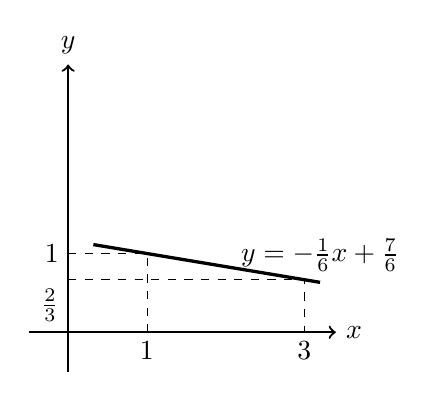
\begin{tikzpicture}[domain = 0.32:3.2, samples = 100, very thick]
        \draw[thick, ->] (-0.5, 0) -- (3.4, 0) node[right] {$x$};
        \draw[thick, ->] (0, -0.5) -- (0, 3.4) node[above] {$y$};
        \draw plot(\x, -1/6 * \x + 7/6) node[above] {$y = -\frac{1}{6}x+\frac{7}{6}$};
        \draw [very thin, dashed] (0,1) node[left]{$1$}--(1,1)--(1,0) node[below]{$1$};
        \draw [very thin, dashed] (0,0.67) node[below left]{$\frac{2}{3}$}--(3,0.67)--(3,0) node[below]{$3$};
    \end{tikzpicture}
    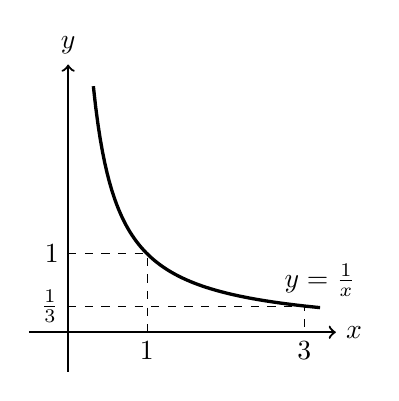
\begin{tikzpicture}[domain = 0.32:3.2, samples = 100, very thick]
        \draw[thick, ->] (-0.5, 0) -- (3.4, 0) node[right] {$x$};
        \draw[thick, ->] (0, -0.5) -- (0, 3.4) node[above] {$y$};
        \draw plot(\x, 1/\x) node[above] {$y = \frac{1}{x}$};
        \draw [very thin, dashed] (0,1) node[left]{$1$}--(1,1)--(1,0) node[below]{$1$};
        \draw [very thin, dashed] (0,0.33) node[left]{$\frac{1}{3}$}--(3,0.33)--(3,0) node[below]{$3$};
    \end{tikzpicture}
    \caption{ボルダ投票の得点重み(選択肢数は6人\protect\footnotemark)}
\end{figure}
\footnotetext{線形な重み付けで,1位の人に1票投票するとすると,候補n人中x位の人への票数$f(x)$は$f(x) = - \frac{1}{n}x + \frac{n+1}{n}$です.}

ナウルのヤレン地区での選挙結果\footnote{Wikipediaから出典を辿ろうとしたら,リンクが切れていました.Wikipedia(https://en.wikipedia.org/wiki/Nauruan\_parliamentary\_election,\_2016i)からの引用になります.}は図32のようになりました.ヤレン選挙区は定数2です.

\begin{figure}[!h]
    \centering
    \begin{tabular}[!h]{|c|c|c|c|c|c|c|c|} \hline
         & 1位 & 2位 & 3位 & 4位 & 5位 & 6位 & 得点 \\ \hline
        Scotty & 255 & 103 &  33 &  24 &  51 &  38 & {\bf 340.03} \\ \hline
        Keke   & 122 &  52 &  46 &  82 &  65 & 137 & {\bf 219.67} \\ \hline
        Eoe    &  71 & 132 &  56 &  51 &  96 &  98 & 203.95 \\ \hline
        Mackay &  11 & 119 & 128 & 123 &  82 &  41 & 167.15 \\ \hline
        Julius &  41 &  35 &  95 & 111 & 118 & 104 & 158.85 \\ \hline
        Amwano &   4 &  62 & 144 & 117 &  91 &  86 & 144.78 \\ \hline
    \end{tabular}
    \caption{ヤレン地区の開票結果}
\end{figure}

図32をよくみると,得点の高い候補は票が上位と下位に分散していて,得点の低い候補は票が中位に集中しています\footnote{同じ選挙の他の選挙区でも同様の結果となっています.}.おそらく,有力な候補というのは支持者も多い傍ら不支持者も多く,泡沫候補はどちらも少ないためにこのような結果になるのでしょう.これはもう人間の心理の問題なのでしょうがないのですが,ボルダ得点法を用いる場合は得点の重み付けを工夫しないと公正さに欠くものになってしまうと言えるでしょう.

\subsubsection*{承認投票方式}
承認投票は,全選択肢を承認する選択肢と承認しない選択肢に分類し,承認する選択肢に1票ずつ投票するという方式です.最も多くの票を得た選択肢が当選します.国連事務総長選挙などで用いられているようです\footnote{日本でも最高裁判所判事の国民審査で使われています.}.

承認投票では各個人はすべての選択肢について吟味を要求します.各選択肢も個人のちょっとした意識や投票行動の変化によって当選の可能性が大きく変動し,強力な候補が落選する可能性も高くなります.これは,承認投票は今まで見てきた投票方式よりも民意を反映しやすいということです.また,贈賄があまり意味をなしません.贈賄して自分の票数が増えても,他の候補の票数が減るわけではないからです.また,各候補に順位を付けるわけではないので,戦略的投票の影響も小さくなります.ちなみに,任意の3選択肢について二分選好になっていることにも注意してください.

そう考えるとなかなかに良さそうな方式に思えます.図33の選好について考えてみましょう.
\begin{figure}[!h]
    \centering
    \begin{tabular}[!h]{|c|c|c|c|} \hline
          & a & b & c \\ \hline
        1 & x & x & z \\ \hline
        2 & y & y & y \\ \hline
        3 & z & z & x \\ \hline
    \end{tabular}
    \caption{個人的選好}
\end{figure}
すべての個人が上位1位の選択肢までを承認した場合はxが選ばれますが,上位2位までを承認した場合はyが選ばれます.例えば事前の世論調査などで予め大体の個人的選好がわかっているときに,「選択肢が4つありますが,上位2選択肢を承認してください.それ以外は無効票とします」というような承認投票を行った場合,結果を思うように操作することもできるかもしれません.

\subsubsection*{パウロスの全員当選モデル}
今まで,様々な多数決方式を見てきました.ここで,パウロスの全員当選モデルという個人的選好に対して各投票方式を当てはめてみたいと思います.図34のパウロスの全員当選モデルでは,5選択肢と55人の個人的選好が定まっています.

\begin{figure}[!h]
    \centering
    \begin{tabular}[!h]{|c|c|c|c|c|c|c|} \hline
           & 18人 & 12人 & 10人 & 9人 & 4人 & 2人 \\ \hline
         1 & x    & y    & z    & u   & v   & v   \\ \hline
         2 & u    & v    & y    & z   & y   & z   \\ \hline
         3 & v    & u    & v    & v   & u   & u   \\ \hline
         4 & z    & z    & u    & y   & z   & y   \\ \hline
         5 & y    & x    & x    & x   & x   & x   \\ \hline
    \end{tabular}
    \caption{全員当選モデル}
\end{figure}

まず,単純多数決ではxが当選します.決選投票だとyが当選.勝ち抜き投票だとzが当選.ボルダ得点で票数を線形に重み付けした時は,x:127点,y:156点,z:162点,u:191点,v:189点でuが当選.逆比例に重み付けした時は,x:25.40点,y:25.35点,z:24.00点,u:26.50点,v:24.33点でuが当選.多数決決定法では循環が生じず,v,u,z,y,xの順に選好し,vが選ばれます.

このように,方式が異なればどの候補も当選しうるということがわかります.結局,多数決で最も好ましい選択肢を選ぶということは,とっても怪しい行いで,多数決と民主制は論理的には全く無関係なものであるというのが事実なのです.

\subsubsection*{結局}
思うに,実際に選挙方式を決めているのはその時の権力者の事情とかその時の社会情勢や民意であって,{\bf どの投票方式が良いとかそういうことではない}のです.パウロスの全員当選モデルのパラドックスが示すように,多数決による意思決定の結果は,一定の公正さはありますが,もはや御神託以外の何者でもないと言ってよいでしょう.

架空世界で社会的決定のルールを決める場合,確かに「ボルダ得点法には操作可能性がある!」や「アローの不可能性定理より完璧な投票方式は存在しない!」というような論理的な主張が影響を与えることもあるでしょう.しかし,たとえ数理的な正しさを大切にする架空世界であっても,時の権力者や政権にとって現在の選挙制度が都合が悪いということが,選挙制度が変わる理由だと考えるべきではないでしょうか.結局,架空世界での選挙制度を考えるときは,公正でない方式を正したり,民意をより反映させたりという点も大事ですが,それよりも,{\bf その時選挙制度を変える権力のある者にとって議会での議席が増えたり意思決定がしやすくなるような決定方法は何か},という点について考えなければ,自然で現実的な架空世界記述ができないように思えます.

また,集計の手間や有権者の意識なども選挙制度に反映されるでしょう.議会の議席配分なら比例代表制だと死票も少なく少数者の意見が反映されやすくあまりパラドックスも生じそうもないので良いと言えるでしょうが,結局,多数決は民主的であることと無関係なわけですし,投票による意思決定にこれと言った解はないようです.

ただ,「この方式はこの世界観と合致しているか?」,「この方式ではパラドックスが生じないか?」などということを考察すると,例えば政治制度を創作する時に根本的な部分から構築ができるし,そのような方式を取るに至る歴史も考察し記述することができると思います\footnote{もともと,これが私が社会的決定理論について調べた一番強い動機です.}.どれが良いとも言えないという事実の中で,なるべく良い方法を探そうとする苦悩はどこの世界にも存在すると思いますし,それを架空の歴史の一側面として想定するなり組み込むなりすると,政治や意思決定の制度に関する創作がよりリアルなものになるでしょうし,凝ったものができるかもしれません\footnote{この文章がそういう作り込みに役立てれば幸いです.}.

ところで,今まで見てきた投票方法は,「投票所に行って,紙にバツとか数字とかを書いて投票して,選挙管理委員の人たちが徹夜して開票作業して,翌朝に結果が出る」というようなものです.どうしても複雑な過程を踏んだり,何度も予備選挙や決選投票などをやるのは金銭的にも厳しいかもしれません.

しかし,例えば情報通信技術の進歩は,投開票の手間を省略してくれるかもしれません.情報技術が進んでいたり,その導入に積極的な架空世界もあるかもしれませんし,そのような考察は何かの役に立つと思っています.最後にそのような場合の投票がどうなるか考えてみたいと思います.


\subsection{投票と技術}
今まで見てきた投票方式にも例えば承認投票や勝ち抜き方式のように票の集計が難しいものがあります.勝ち抜き方式では選択肢の数(n個) $\times$ 個人の数(m個)のデータを扱う必要があります.この場合各投票用紙のn個のデータをm回集計したあと順番に並べるので,$O(mn)$の時間計算量です.多項式時間で集計できないような方式なら別ですが,この場合,電子投票ならば集計が一瞬で終わります.そうすると,今まで選挙にまとわりついていた様々な制約が消え,選挙制度や政治制度の変革が起こりえます.

また,架空世界創作という観点に立てば,情報通信技術でできることは魔法でもできるかもしれません.魔法世界での社会的決定で我々が行っているような単記投票ばかりが用いられていると考えるのはむしろ不自然なのかもしれません.具体的に魔法がどのようなものかについての考察はしませんが,魔法のある架空世界の創作者は,その世界の魔法が情報や通信に応用できるならどのように投票にも応用できるのかを考えてみるといいかもしれません.

一般にどのような組織も自分で自分を規制するルールを制定することには消極的なので,一票の格差是正などの問題を国会の議論だけに任せてもその場しのぎの対策だけで済まされてしまうことでしょう.選挙制度を決めるのが人間である限りは選挙制度改革はなかなか進みません.情報技術の進歩した社会においては選挙制度の決定も機械的に処理されるものだと考えるべきでしょう.

\subsubsection*{オンライン投票と集計作業の自動化}
有権者がパソコンや携帯端末を用いて投票することについて考えてみましょう.

最初に問題になるのはすべての有権者がパソコンや携帯端末を保有しているのかという問題です.当然ですが,有権者のほぼ全員が情報通信機器にアクセスできなければ電子投票は不可能です.現在の日本では携帯端末機器の世帯保有率は9割を超えていています\footnote{情報通信白書 平成29年度版 第1部 第1章 第1節 図1-1-1-1}.SFなどで出てくる世界観や科学技術観はその当時の水準に影響されるように思いますし\footnote{特に根拠はないですが.},現在含め今後,架空世界創作の中でほぼすべての有権者が携帯端末を保有し操作できる架空世界が多数現れることは想像に難くないでしょう\footnote{というか,すでにそういう世界観の作品は多数あるっぽいです.}\footnote{そのような世界では,携帯端末を保有していないことが経済的格差の象徴とされるかもしれません.格差のあり方によっては携帯機器不保持で個人認証ができないために投票できないということも考えられます.まあ,創作という観点から見るとそのような層を登場させないことで格差を隠すこともできますが,投票という観点から見ると考慮すべき事案かもしれません.}.そのような世界では,電子投票・オンライン投票の利点が大きそうです.利点について考えてみましょう.

まず,有権者が自分の携帯端末から投票するならば,自治体は多数の投票所を設置する必要もありませんし,開票作業に多額の人件費をかける必要もありません.現在,日本では一回の国政選挙で全国約5万箇所の投票所が必要で\footnote{http://www.soumu.go.jp/senkyo/48sansokuhou/index.html},選挙のたびに600億円以上もの費用がかかります\footnote{http://www.soumu.go.jp/main\_content/000506000.pdf}.さらに有権者が投票所に出向く必要もなくなります.投票所に出向く必要があると,投票日に雨が降ったりすると投票率が落ちたりするので,どこでも投票できるのは利便性だけでなく,投票率向上の効果も期待できそうです.携帯端末からの投票なので,全国どこからでも,国外からでも容易に投票が可能です.投票期間を一日に限定せず,長めに取ることもできます\footnote{この場合,すでに投票した個人が期日前に死亡すると投票は無効になるんでしょうか?}.また,投票の内容を期日中ならなんどでも変更するということも可能です.これは,他人による意志の強要などの回避にもつながります.便利で気軽に投票できるシステムであれば,社会的決定への参加がより身近になり,投票率向上などの様々な利点があると考えられます.他にも,無効票の投票がシステム的に不可能など,無数に利点が挙げられるのではないでしょうか.

投票においては不正投票の防止のために個人認証が必要になります.指紋や声紋などでの認識など様々な方法が考えられます.情報通信機器による個人認証はなりすましが容易なのではないかとも考えられますが,日本の国政選挙で行われているハガキと立会人の目視\footnote{性別や年齢などを確認するらしいです.}による本人確認も,誰が住んでるかよくわからない都会でなら同様になりすましが容易でしょうし,電子投票の方がなりすましが困難なような認証方法も考えられるでしょうから,個々の架空世界の技術でなんとかなると思うので,なんとかしてください.

集計もすべて自動化が可能となり,人選費の削減や開票作業が正確で高速なものになります.必要な人手はシステムの起動や開票結果の公表程度です.コスト全体ではシステムの運用・保守のためのコストが最も大きな割合を占めるでしょうが,人力でやるのに比べると僅かなものです.選挙期間中に自治体の業務が増えることもなく,職員の休日出勤も不要になります.

\subsubsection*{区割りの最適化による格差是正}
多数の議員を選出する時,共同体全体を地域や部族などに分ける選挙区を導入することがあります.この時問題となるのが,一票の格差や特定の候補に有利になるような区割り\footnote{いわゆるゲリマンダーです.}がされたりすることです.人間が区割りをする以上は様々な思惑が介入するでしょうし,区割りも自動的に決めるべきという考え方もできるかもしれません.

一票の格差を是正するためには,すべての選挙区の有権者数を一定の範囲内に収める必要があります\footnote{なるべく,$\frac{全有権者数}{議員定数}\times 選出議員数に近づくようにします.$}.この場合,地域全体を地域特性等を考慮して数百人・数千人規模ごとに分割し,適切に併合していくという組み合わせ最適化問題とすればよいでしょう\footnote{人口統計調査や人種分布・言語分布などをもとに少数者に不利にならないようにしながら,なるべく区割りが歪な形にならないようにするとよいかもしれません.}.このような区割りを選挙前に自動的に行い,選挙運動が始まる前に公表することになります.

選挙制度改革でこのように区割りの最適化を毎回行うというのは,多くの議員にとって好ましいことではないでしょう.なぜならば,議員にはその選挙区の有権者との密接な人間関係があるかもしれないからです\footnote{いわゆる地盤です.}.機械的な区割りの決定によって既存の選挙区と大きく区画が変わった場合,今まで当選確実だった候補が再選を果たせなくなることも考えられます.そのことも考慮すれば,選挙の後に次の選挙で用いる区割りを予め決めておくという方法も有効かもしれません.ただ,民主的社会であるならば,個人の平等性,すなわち一票の格差が少ない状態であることは優先されるべきですし,個々の議員の地盤に配慮するべきではないのかもしれません.いくら有能な人材であっても,多数の支持を得られなければ選出されないのは仕方がないことではあります.

\subsubsection*{シュルツ方式}
単記投票の開票・集計作業の時間計算量は選択肢mつ,個人n人とすれば,$O(n)$です.ボルダ得点でも$O(mn)$です.一方,多数決決定法だと$O(m^2 n)$です\footnote{選択肢のペア$_mC_2 = \frac{m(m-1)}{2}$個に対する個人的選好をn人分集計するので.}.$O(n^2)$のような方式はあまりないと思いますが,もしそのような方式があれば,$n = 1,000$ともなれば,開票作業は人力では到底一晩では終わりません.しかし,電子投票で集まったデータを集計するなら,この程度はすぐ終わります.

シュルツ方式という方式があります.多数決決定法のように個人の選好をすべて反映させますが,社会的選好が非循環性を満たす方式です.多数決決定法では2選択肢のどちらを選好する個人が多いかで社会的選好を決めます.しかし,それだと社会的に循環が起こりますが,シュルツ方式では様々な選択肢間の選好まで見て循環しないように社会的選好を決めて循環を回避しています.

シュルツ方式では,2選択肢間の道と,その道の強さというものを考えて社会的決定をします.

\begin{dfn}
    $d(x,y)$は$x>y$と選好する個人の数です.    
\end{dfn}
\begin{dfn}[道]
    選択肢$x_0$から$x_{n-1}$への道とは,$\forall i (d(x_i,x,{i+1}) > d(x_{i+1},x_i))$を満たすような異なるn個の選択肢$x_0,x_1,\dots,x_{n-1}$の列のことです.
\end{dfn}
ただし,始点と終点が同じであるような道について考えるときだけは,始点と終点の重複を許すことにします.
\begin{dfn}[道の強さ]
    選択肢$x_0$から$x_{n-1}$への道において道の強さとは,\\$d(x_0,x_1),d(x_1,x_2),\dots,d(x_{n-2},x_{n-1})$の最小値のことです.そのような道が存在しない場合は強さを0とします.
\end{dfn}
\begin{dfn}
    選択肢$x$から$y$への道の強さの最大値を$p(x,y)$とします.
\end{dfn}
\begin{dfn}[シュルツ方式]
    シュルツ方式とは,社会的選好を
    \begin{equation*}
        x \succeq y \leftrightarrow p(x,y) \geq p(y,x)
    \end{equation*}
    とする決定方式のことです.
\end{dfn}

個人的選好を図35のようにします.
\begin{figure}[!h]
    \centering
    \begin{tabular}[!h]{|c|c|c|c|c|c|} \hline
          & 8人 & 2人 & 4人 & 4人 & 3人 \\ \hline
        1 & x   & y   & z   & w   & w   \\ \hline
        2 & z   & x   & w   & y   & z   \\ \hline
        3 & w   & w   & y   & x   & y   \\ \hline
        4 & y   & z   & x   & z   & x   \\ \hline
    \end{tabular}
    \caption{個人的選好}
\end{figure}
このとき,すべての選択肢のペアに対して図36のようになります.
\begin{figure}[!h]
    \centering
    \begin{tabular}[!h]{|c|c|c|c|c|} \hline
               & d(*,x) & d(*,y) & d(*,z) & d(*,w) \\ \hline
        d(x,*) &        &  8     & 14     & 10     \\ \hline
        d(y,*) & 13     &        &  6     &  2     \\ \hline
        d(z,*) &  7     & 15     &        & 12     \\ \hline
        d(w,*) & 11     & 19     &  9     &        \\ \hline
    \end{tabular}
    \caption{$d(*,*)$}
\end{figure}

2選択肢について,選好する人が少ない選択肢を始点,多い選択肢を終点とする辺による有向グラフを考えれば,道の強さ$p(x,y)$はそのグラフでxからyへの道での途中の辺の強さの最小値となります.
\begin{figure}[!h]
    \centering
    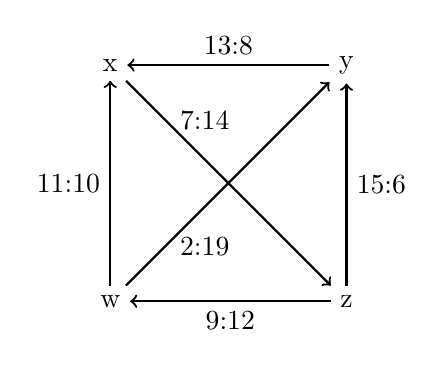
\begin{tikzpicture}
        \node (x) at (0,3) {x};
        \node (y) at (3,3) {y};
        \node (z) at (3,0) {z};
        \node (w) at (0,0) {w};
        \draw[thick, <-] (x) -- node[above]{13:8} (y);
        \draw[thick, ->] (x) -- (z);
        \draw[thick, <-] (x) -- node[left]{11:10} (w);
        \draw[thick, <-] (y) -- node[right]{15:6} (z);
        \draw[thick, <-] (y) -- (w);
        \draw[thick, ->] (z) -- node[below]{9:12} (w);
        \node (1) at (1.2,2.3) {7:14};
        \node (2) at (1.2,0.7) {2:19};
    \end{tikzpicture}
    \caption{グラフ}
\end{figure}
グラフは図37のようになります.図37より,図38のようになります.
\begin{figure}[!h]
    \centering
    \begin{tabular}[!h]{|c|c|c|c|c|} \hline
               & p(*,x) & p(*,y) & p(*,z) & p(*,w) \\ \hline
        p(x,*) &        & 14     & 14     & 12     \\ \hline
        p(y,*) & 13     &        & 13     & 12     \\ \hline
        p(z,*) & 13     & 15     &        & 12     \\ \hline
        p(w,*) & 13     & 19     & 13     &        \\ \hline
    \end{tabular}
    \caption{$p(*,*)$}
\end{figure}
図38より,$w \succ x \succ z \succ y$です.

ところで,図35$\sim$図38の例では社会的選好に推移性と非循環性が成立していることが確認できますが,どのような場合でも推移性や非循環性が成立しているのでしょうか?

推移性は満たしていません.例えば,$x > y > z, x > z > y, y > x > z, z > y > x$とする個人が1人ずついる場合,$p(x,y) = p(y,x) = p(y,z) = p(z,y) = p(z,x) = 2$ですが,$p(x,z) = 3$となり,$x \simeq y \land y \simeq z$なのに,$x \succ z$となり,推移性は満たしません.

非循環性は常に成立することが証明できます.そのことを証明する前に少しシュルツ方式の性質について述べることにします.

\begin{lem}
    シュルツ方式では,任意の異なる3選択肢x,y,zに対して,
    \begin{equation*}
        min\{p(x,y),p(y,z)\} \leq p(x,z)
    \end{equation*}
    が成り立ちます.また,
    \begin{equation*}
        p(x,y) \leq p(x,z) \lor p(y,z) \leq p(x,z)
    \end{equation*}
    が成り立ちます.
\end{lem}
\begin{proof}
xからzへ至るすべての道の強さの最大値が$p(x,z)$です.ここで,xからyへ至る強さ$p(x,y)$の道とyからzへ至る強さ$p(y,z)$の道がともに存在するならば,それらを合わせた道の強さは$min\{p(x,y),p(y,z)\}$となります.xからzへ至る道の強さは$p(x,z)$以下なので,$min\{p(x,y),p(y,z)\} \leq p(x,z)$となります.xからyへの道かyからzへの道のどちらかまたは両方が存在しない場合は,$min\{p(x,y),p(y,z)\} = 0$なので,条件は常に成立します.

$min\{p(x,y),p(y,z)\} \leq p(x,z)$から,それと同値な命題$p(x,y) \leq p(x,z) \lor p(y,z) \leq p(x,z)$が成り立つこともわかります.
\end{proof}

次に述べるのはシュルツ方式の説明ではないですが,シュルツ方式の性質を証明するのに使うものです.
\begin{dfn}[擬推移性]
    任意の二項関係$R$は,任意の3つの選択肢の組$x,y,z$に対して,$xPy \land yPz \to xPz$を満たすとき擬推移性を持つと言います.ただし,$P$は,$xPy \leftrightarrow xRy \land \sim yRx$です.
\end{dfn}
$R$が$\geq,\succeq$,$P$が$>,\succ$に対応します.
\begin{lem}
    推移性を持つ二項関係は擬推移性も持ちます.また,擬推移性を持つ二項関係は非循環性も持ちます.
\end{lem}
\begin{proof}
(推移性$\to$擬推移性)二項関係$R$が推移性を持つとします.この時,$xPy \land yPz \to xPz$を示せば良いので,前件$xPy \land yPz$を仮定します.推移性より,$xPy \land yPz \to xRy \land yRz \to xRz$.$zRx$を仮定すると,推移性より$zRx \land xRy \to zRy$.しかし,$yPz$より矛盾.よって,背理法より$\sim xRz$です.よって$xPz$となり,$R$は擬推移性も満たします.

(擬推移性$\to$非循環性)二項関係$R$が擬推移性を持つとします.この時$n$個の選択肢$x_1,\dots,x_n$に対して,数学的帰納法より$x_1 P x_2 P \dots P x_n \to x_1 P x_n$です.よって,$x_1 P x_2 P \dots P x_n \to x_1 R x_n$なので,非循環性も満たします.
\end{proof}


\begin{thm}
    シュルツ方式は個人的選好の自由を満たす社会的決定関数です.
\end{thm}

\begin{proof}
シュルツ方式で,どのような選択肢の組に対しても,反射性,完全性,非循環性が成り立つことを示せばよいです.

(反射性)任意の選択肢xに対して,$p(x,x) = p(x,x)$なので,当然$x \succeq x$です.

(完全性)任意の異なる2つの選択肢x,yに対して,整数$p(x,y)$と$p(y,x)$が存在し,$p(x,y) < p(y,x)$または$p(x,y) = p(y,x)$または$p(x,y) > p(y,x)$であり,よって,$x \prec y$または$x \simeq y$または$x \succ y$です.

(非循環性)補題6.2より,擬推移性を満たすことが示せれば良いです.$x \succ y \land y \succ z$を仮定します.この時,$p(x,y) > p(y,x)$かつ$p(y,z) > p(z,y)$です.$x \succ z$を示したいので,$p(x,z) > p(z,x)$となれば良いです.

補題6.1より,$p(x,y) \leq p(x,z) \lor p(y,z) \leq p(x,z)$.$p(x,y) \leq p(x,z)$の時について考えます.この時,$p(x,z) \geq p(x,y) > p(y,x)$です.

補題6.1より,$p(y,z) \leq p(y,x) \lor p(z,x) \leq p(y,x)$.$p(z,x) \leq p(y,x)$の時,$p(x,z) > p(y,x) \geq p(z,x)$より,$x \succ z$です.$p(y,z) \leq p(y,x)$の時,$p(y,z) > p(z,y)$より,$p(x,z) \geq p(x,y) > p(z,y)$です.補題6.1より,$p(z,x) \leq p(z,y) \lor p(x,y) \leq p(z,y)$です.$p(x,y) \leq p(z,y)$の時は,$p(x,y) > p(x,y)$で矛盾します.よって,$p(x,y) \not \leq p(z,y)$とわかり,選言三段論法より$p(z,x) \leq p(z,y)$です.よって,$p(x,z) > p(z,x)$で,$x \succ z$です.

$p(y,z) \leq p(x,z)$の時についても図39の手順を追えば同様に示すことができます.よって非循環性も満たします.

\begin{figure}[!h]
    \centering
    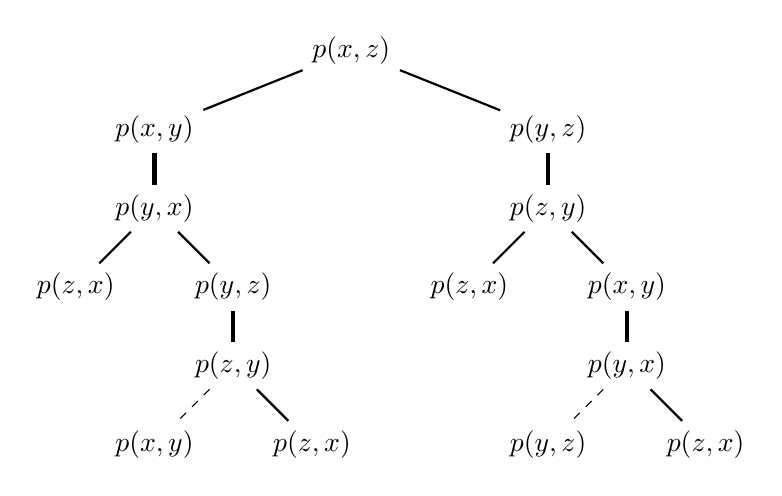
\begin{tikzpicture}
        \node (a) at (3.5,5){$p(x,z)$};
        \node (b) at (1,4) {$p(x,y)$};
        \node (c) at (1,3) {$p(y,x)$};
        \node (d) at (0,2) {$p(z,x)$};
        \node (e) at (2,2) {$p(y,z)$};
        \node (f) at (2,1) {$p(z,y)$};
        \node (g) at (1,0) {$p(x,y)$};
        \node (h) at (3,0) {$p(z,x)$};
        \node (i) at (6,4) {$p(y,z)$};
        \node (j) at (6,3) {$p(z,y)$};
        \node (k) at (5,2) {$p(z,x)$};
        \node (l) at (7,2) {$p(x,y)$};
        \node (m) at (7,1) {$p(y,x)$};
        \node (n) at (6,0) {$p(y,z)$};
        \node (o) at (8,0) {$p(z,x)$};
        \draw[thick]       (a) -- (b);
        \draw[ultra thick] (b) -- (c);
        \draw[thick]       (c) -- (d);
        \draw[thick]       (c) -- (e);
        \draw[ultra thick] (e) -- (f);
        \draw[dashed]      (f) -- (g);
        \draw[thick]       (f) -- (h);
        \draw[thick]       (a) -- (i);
        \draw[ultra thick] (i) -- (j);
        \draw[thick]       (j) -- (k);
        \draw[thick]       (j) -- (l);
        \draw[ultra thick] (l) -- (m);
        \draw[dashed]      (m) -- (n);
        \draw[thick]       (m) -- (o);
    \end{tikzpicture}
    \caption{証明の手順(太線は$>$,細線は$\geq$,点線は矛盾を表します.)}
\end{figure}
\end{proof}
図39から,推移性を満たすだけ,すなわち太線が細線になる時は,点線部分の矛盾が示せないことがわかります.このことからシュルツ方式は社会的には推移性を満たさないことがわかります.逆に,$x \succeq y \succ z \to x \succ z$のような擬順序より弱い条件でも満たすこともわかります.

シュルツ方式は社会的決定関数なわけですから,必ず選択集合が存在します.つまり,投票を行って最良要素を選ぶことができます.これは社会的決定には十分な性質と言えます.

では,シュルツ方式の開票・集計作業の時間計算量はどれだけになるでしょうか.投票データから$d(*,*)$を表にするのに$O(m^2 n)$.$p(*,*)$の表を作るのが少しむずかしいですが,ワーシャル・フロイド法というアルゴリズムを用いれば$O(m^3)$で計算できることが知られています.$p(*,*)$の表から社会的選好を決めるのには$O(m^2)$なので,結局,$O(m^2 n + m^3)$です.

単記投票法が$O(n)$なので,選択肢が数倍程度に増えても単記投票法では手間が大して変わらないのに対して,シュルツ方式は選択肢の増加率のべきに比例する量の開票作業が必要になります.しかし,選択肢の数が急増するとしても高々10倍程度まででしょうし,計算機を用いて開票することを考えればシュルツ方式は集計が不可能な方式ではありません.

シュルツ方式は欠点が少ない方式として知られていて\footnote{無関係選択肢からの独立性は満たしていません.しかし,思うにこれほど複雑な方式だと戦略的投票ができるんだろうかという感じもしますし,あまり大きな欠点ではないのかもしれません.},Debianやウィキメディア財団,Haskellなどで投票方式として使われています.すごそうな方式なのですが,その利点について深く述べることはちょっと大変なのでやめます.詳しいことを知りたい人は参考文献[4]などを参考にしてください.ここで述べたいのは,時間計算量が$O(m^2 n)$のような多数決方法も情報通信機器を利用して電子投票すれば可能だということです.電子投票をする世界では,投票方式についてもこのように多様な選択が可能となります.

\subsection{電子投票な世界はどうなのか}
今まで色々見てきました.現実世界でも電子投票が導入されれば良いのになあという思いもあるわけですが,時期尚早と言われれば,まあそうですね,という感じもします.架空世界ならば電子投票を導入することに積極的な世界もあるでしょうが,そもそも電子投票をする世界では投票だけではなく,メディアによる世論の形成や国民的議論も情報通信機器によってなされるかと思われます.

多数決が民主的とは無関係であること,民主制にとって重要なのは議論と交渉(なのではないか)ということはすでに述べたとおりです.この文書では社会的決定方式の方に重きを置いていますが,それは理論やシステムの話であって,実際に理念として大切なのは意思決定に参加する個々人の意識なのだろうと思います.一体どのようにすれば多様な意見を比較検討するような意思決定ができるのか,個々の架空世界の世界観が大きく反映されるところでしょうし,大雑把にしか述べられませんし,私の稚拙な考えがどこまで役に立つかはわかりませんが,少しだけ考えてみたいと思います.

どれだけ議論を重視するような文化であろうと,誰しもが積極的に議論や交渉に参加できるわけではありません.しかし,そのような人々の意見も民主的な社会的決定には当然反映されるべきです.そこで,投票と議論を段階的に繰り返していくという手法が考えられます.何度も投票・議論を繰り返すことは我々の住む現代においても時間と費用がかかる非常に困難なことですが,情報通信技術が高度に発達した世界では,小規模な投票行為や議論は日常的に行われていることなのかもしれません.そのような場合,社会全体としての意思決定も,予備の投票を事前に行うなどして社会全体の個人的選好の状態などを把握,分析し,個人的選好を洗練させてからまた投票を行うという過程が重視されることも考えられます.

情報通信機器が高度に発達した社会では,広告などの技術も発達していることが想定されます.視線を誘導したり,意識を操作するような広告があっても不思議ではありません.個人的選好の変化がそのような資本や社会による操作によって変化する社会が民主的と言えるかは怪しいところです.そう考えると,資本や社会の思惑などにも批判的な目が向けられたり,社会的な議論を喚起することができる自由な言論空間の存在がなければ,安定的な意思決定は不可能なのかもしれません.

この程度を述べるに留まりたいですが,架空世界における意思決定というのは,個人的には考えれば考えるほど難しいなあという感じです.そもそも,架空世界の社会的決定は創作者の思想の問題なのかもしれないので,あまり私が持論を述べた所で意味がないかもしれませんが,少しでも共感できたり参考にしていただけるところがあれば,嬉しい限りです.



\section{最後に}
部分的に読んでくださった方も,全体的に読んでくださった方も,ここまで読んでいただいて本当にありがとうございます.架空世界における歴史や数学や科学等の考察は架空世界創作をしている方々のコミュニティーを覗くとたびたび観察されますが,ここまで述べたような社会的決定という観点についてはあまり考慮されていないように思います.もし,この文書を読んで何か思うところがあったり,ここで述べた投票方式の例などを使ってみよう程度でも何でも,架空世界創作に少しばかり応用してみようというふうに思っていただけたらとても嬉しい限りです.

最初この文書を書き始めたときは,「20ページぐらいで終わるだろうし,1週間もあれば余裕で書けるだろうなあ」と思っていたのですが,思っていたより書くべきことが多く,60ページを超える分量になってしまいました.さらに,私の能力不足と怠惰さも相まって1ヶ月近くの執筆期間を要してしまい,貴重な春休みの多くの時間を費やすことになってしまいました\footnote{ふええ.}.

ここで述べたことは,いわゆる社会的決定理論の話になるのかと思います.しかし,私は情報系の学生で,別に経済学や経営工学の学生ではないので,専門的に学んでいるわけではありません.至らぬところが多々あると思いますが,架空世界創作における理論的考察に貢献したいという思いから,頑張って書きました.もし,間違い等のご指摘があれば,Twitter:@nymwaへお願いします.

\begin{thebibliography}{99}
    \bibitem{Sai01} 佐伯 胖, 「きめ方」の論理 社会的決定理論への招待,1980.
    \bibitem{Mat01} 松本 保美,アローの不可能性定理 枠組みの検討と応用可能性,2013.
    \bibitem{Sen01} A. Sen,
    Collective Choice and Social Welfare : Expanded Edition, 2017.
    \bibitem{Sch01} M. Schulze, A New Monotonic, Clone-Independent, Reversal Symmetric, and Condorcet-Consistent Single-Winner Election Method (http://m-schulze.9mail.de/schulze1.pdf), 2017.
\end{thebibliography}
\end{document}



